% Appendix Template

\chapter{GRB and afterglow theory} % Main appendix title

\label{app:afg} % Change X to a consecutive letter; for referencing this appendix elsewhere, use \ref{AppendixX}

This chapter is based in the \cite{Kumar:2014upa} work.

\section{Theoretical background}

This section aims to outline a brief overview of the most relevant physical processes in GRBs. Tt is not meant as a comprehensive theoretical review. For this we refer the interested reader to the momnograph by \citet{RybickiLightman:1985}, as well as books of high energy astrophysics by \citet{Longair:2011,Dermer:2009}.

In this section we focus first on certain aspects of theory of special relativity, and relativistic hydrodynamics 
\red{this is where you put the NAVA and Peer models for dynamcs, Sedov Teylor and stuff maybe 
    and on radiation processes, synchrotron, \red{inverse-Compton} and \red{photon-pion} processes.
}


\subsection{Special relativistic effects}

\begin{figure*}[t]
    \centering 
    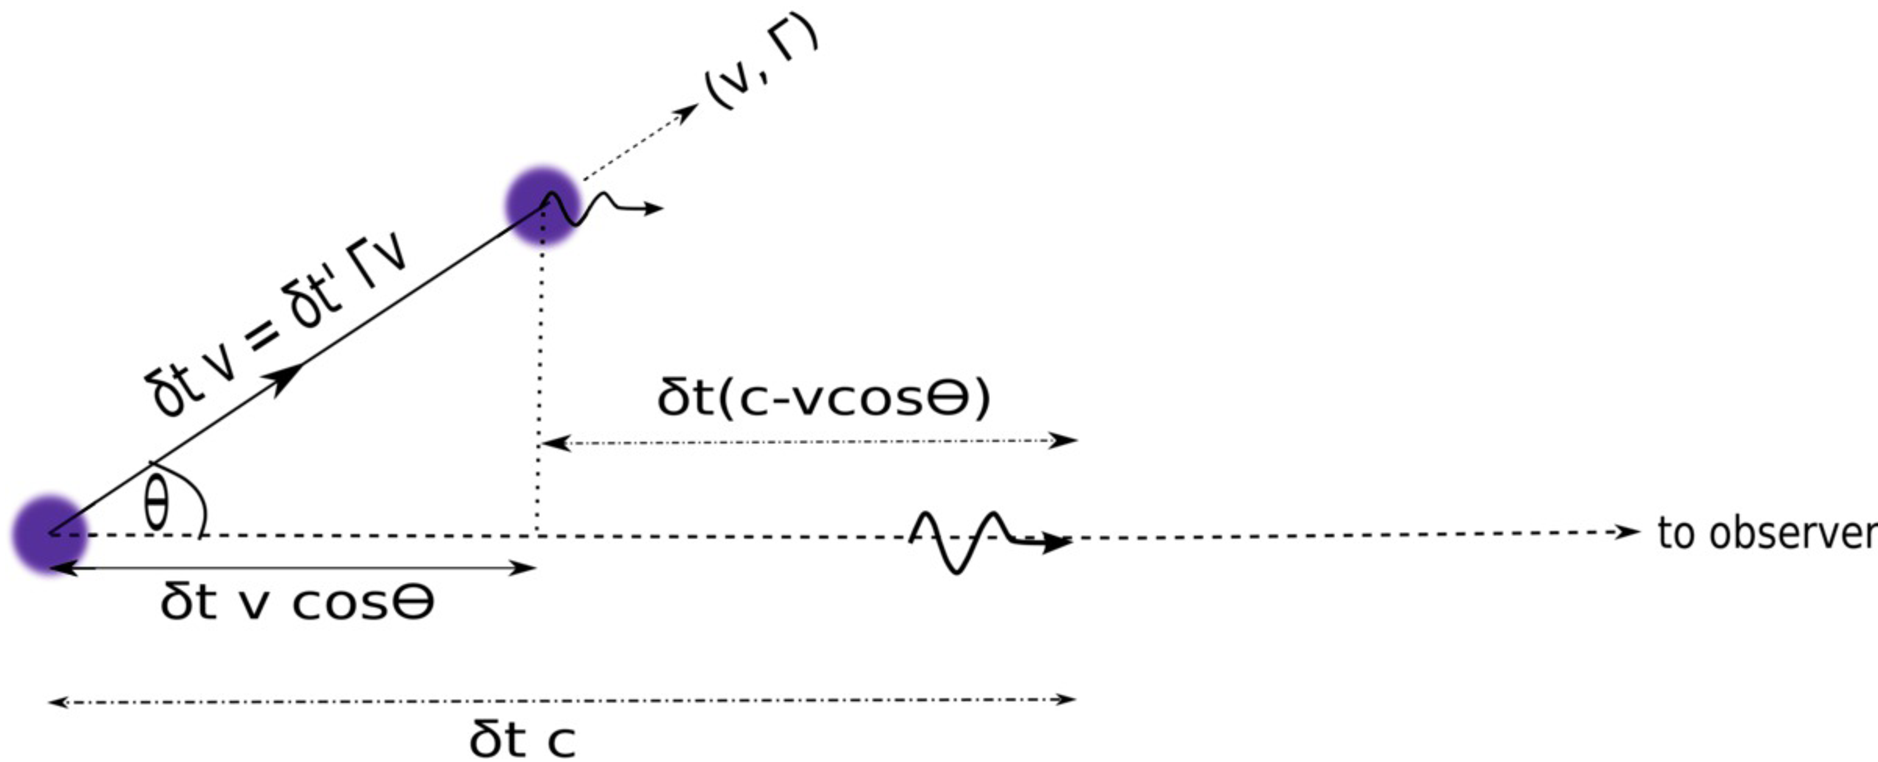
\includegraphics[width=0.45\textwidth]{Fig_1_KZ.pdf}
    \caption{
        The relation between pulse duration in source comoving frame, $\delta t'$, lab frame
        $(\delta t)$, and the time interval for pulse received by a distant observer is shown in this figure. The source is moving with speed $\upsilon$ (Lorentz factor $\Gamma$), at an angle $\theta$ with
        respect to observer line of sight. One photon is emitted when the source was at the
        location at the left side of the figure. And a second photon is emitted $\delta t'$ later when
        the photon has already traveled a distance $c\Delta t$ toward the observer, and the source
        is also a distance $\upsilon$ cos $\theta\delta t$ closer. The difference between these two distances is the
        time interval in the observer frame for the arrival of the two photons which is given
        by equation 1.
        (Adapted from \citet{Kumar:2014upa}, Fig.~1)
    }
    \label{fig:aafg:theory:sr1}
\end{figure*}

Consider a moving source of radiation and an observer with a line of sight to the source. Let $\upsilon$, $\Gamma$ and $\theta$ be the source velocity, \ac{LF} and angle with the line of sight. \red{REPLACE $\theta$ with $\Phi$ for consistency! (remember spreading jet)}

Consider three frames of reference, the comoving frame (usually denoted with a prime $'$), the lab frame, where the source is seen as moving with $\upsilon$ and observer frame. Then, if two photons are emitted in the comoving frame with time difference of $\delta t'$, which is in the lab frame $\delta t = \Gamma \delta t'$, the observer sees the two photons arrive with 

\begin{eqnarray}
\delta t_{obs} &= \delta t + \frac{(d - \upsilon\cos(\theta) \delta t)}{c} - \frac{d}{c} \\
&= \delta t (1 - \upsilon \cos(\theta) / c) \\
&= \delta t' \Gamma (1 - \upsilon \cos(\theta) / c)\\
&= \delta t' \mathcal{D}^{-1}
\end{eqnarray}

where $d$ is the distance to the source, and 

\begin{equation}
\mathcal{D} = \frac{1}{\Gamma(1 - (\upsilon/c) \cos(\theta))} = \frac{1}{\Gamma(1 - \beta\cos(\theta))}
\end{equation}

is the \ac{DF}. 
\gray{Note that if $\theta \ll 1$ and $\Gamma \gg 1$, the $\delta t_{obs} \approx (\delta t' / \Gamma) (1 + \theta^2 \Gamma^2)/2 = (\delta/\Gamma^2)(1 + (\theta\Gamma)^2/2)$}.
See Fig.~\ref{fig:aafg:theory:sr1}.

Next, we consider the transformation of the photon frequencies. 
Once again $\nu'$ denotes the frequency in the comoving frame and $\nu$ denotes the frequency in the observer frame. 
We employ the standard Lorentz transformation of the photon $4$-momentum in comoving frame, \eg,, $\nu'(1, \cos(\theta'), \sin(\theta'),0)$ to the lab frame $4$-momentum $\nu(1, \cos(\theta), \sin(\theta), 0)$

\begin{equation}
\nu = \nu' \Gamma(1+\upsilon \cos(\theta')/c) \text{ \& } \nu\cos(\theta) = \nu' \Gamma (\cos(\theta') + \upsilon/c)
\end{equation}

or 

\begin{equation}
\nu = \frac{\nu'}{\Gamma (1 - \upsilon\cos(\theta)/c)} = \nu' / \mathcal{D}
\end{equation}

which is a standard Doppler shift formula.
\red{This formula is used in the Code to convert given frequency into the comoving one}


\subsubsection{Relativistic beaming of photons}

We have shown that $\nu = \nu' \mathcal{D}$, but also $\sin(\theta) = \sin(\theta')/\mathcal{D}$. Then the transverse component of the momentum is invariant under the Lorentz transformation, \eg, $\nu_{\perp}' = \nu'\sin(\theta') = \nu\sin(\theta) \nu_{\perp}$. 
For a beem of photons it imples that the angular size of the beem is smaller in the lab frame than in the comoving frame by $\propto \Gamma$.
The solid angle of a conical beem of photons, $d\Gamma$ then 

\begin{equation}
d\Gamma = \sin(\theta)d\theta d\phi = \sin(\theta') d\theta' d\phi' / \mathcal{D}^2 = d\Omega'/\mathcal{D}^2
\end{equation}

is smaller in the lab frame than in the comoving frame.

Next, consider a frequency integrated total energy radiated per init time over the $4\pi$ steradians, denoted as $P$. 
\gray{Assume that the photon been is symmetric under the parity transformation in particle rest-frame (energy radiated per unit of the solid angle in $\theta\phi$ and $\pi-\theta,\pi+\phi$ are the same} \red{assume emission is locally isotropic.}.
%% ---
The the power in the lab frame $P = P'\Gamma\delta t'/(\Gamma\delta t') = P'$. 
Hence, power radiated by particles is \magenta{Lorentz invariant}.


\subsubsection{Transformation of specific luminosity and specific intensity}

Consider a spherically symmetric source, expanding with Lorentz factor $\Gamma$. 
%% ---
Introduce the \magenta{specific luminosity}, defined as the total energy that passes through the surface enclosing the source per unit time, per unit frequency, $L_{\nu} = dE / d\nu dt_{obs}$. 
As $d\nu dt_{obs} = d\nu' dt'$ and $E=\Gamma E'$, the Lorentz transformation of luminosity is

\begin{equation}
L_{\nu} = \frac{dE}{d\nu dt_{obs}} = \Gamma \frac{dE'}{d\nu' dt'} = \Gamma L_{\nu}'
\end{equation}

assuming that the $3$-momentum is zero (as the source is spherically symmetric).

Next, introduce the \magenta{specific intensity}, defined as a flux per unit frequency and per unit solid angle, mediated by photons, transversing surface $dA$, perpendicular to the conical beam, confining the photons, 

\begin{equation}
I_{\nu} = \frac{dE}{d\nu dt_{obs} dA d\Omega}
\end{equation}

that has a Lorentz transformation $I_{\nu} = \mathcal{D}^3 I_{\nu'}'$ as $d\nu dt_{obs} dA$ is the Lorentz invariant.


\subsubsection{Observed \ac{LC} from a source that is suddenly turned off}

\begin{figure*}[t]
    \centering 
    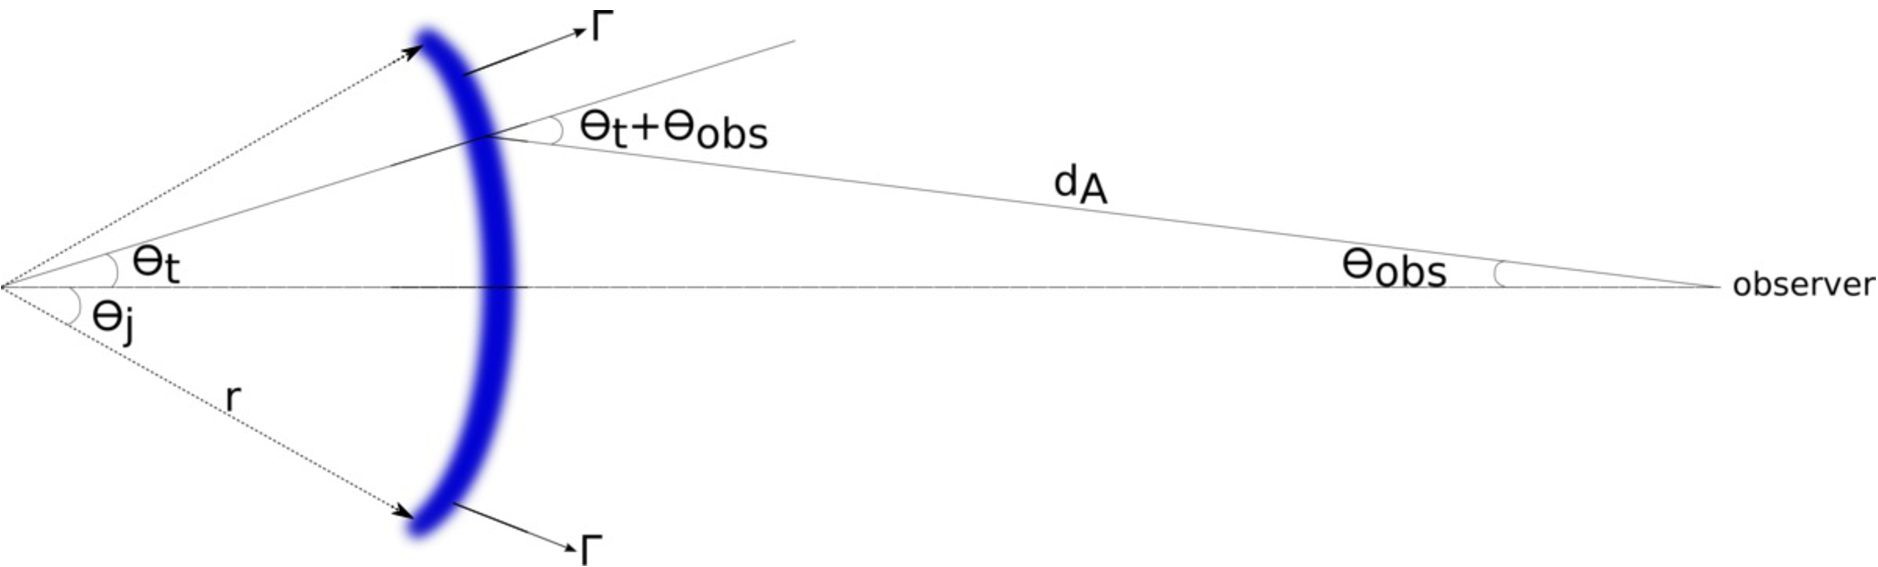
\includegraphics[width=0.45\textwidth]{Fig_2_KZ.pdf}
    \caption{
        The relation between pulse duration in source comoving frame, $\delta t'$, lab frame
        $(\delta t)$, and the time interval for pulse received by a distant observer is shown in this figure. The source is moving with speed $\upsilon$ (\ac{LF} $\Gamma$), at an angle $\theta$ with
        respect to observer line of sight. One photon is emitted when the source was at the
        location at the left side of the figure. And a second photon is emitted $\delta t'$ later when
        the photon has already traveled a distance $c\Delta t$ toward the observer, and the source
        is also a distance $\upsilon$ cos $\theta\delta t$ closer. The difference between these two distances is the
        time interval in the observer frame for the arrival of the two photons which is given
        by equation 1.
        (Adapted from \citet{Kumar:2014upa}, Fig.~1)
    }
    \label{fig:aafg:theory:sr2}
\end{figure*}

\red{it mainly says that when the source turns off, because of its finite angular extend and EATS, the observed flux does not switches off, but rapidly declies.}

Considering the variability of \ac{EM} transients such as \ac{GRB} it is important to asses how a sudden turn off of the source affects the observed emission. 
Consider a relativist thin shell moving within a cone with \ac{LF} $\Gamma$. As it reaches the radius $r=R_0$ the source turns off. 
\red{
    A point on the thin shell is characterized by $(r,\theta,\phi)$ where $\theta$ is the angle measured with respect to the line of sight to the observer. Then, photons, emitted at $(r=\upsilon t, \theta,\phi)$ arrive at the observer with a time delay with respect to a photon emitted at $r=0$ of
}

\begin{equation}
t_{obs} = t - \frac{r \cos(\theta)}{c} = t(1-\frac{\upsilon\cos(\theta)}{c}) = \frac{t}{\Gamma\mathcal{D}}
\end{equation}

Now, consider the observed emission from the source at frequency $\nu$. The starting time is $t_{0;obs}\approx(R_02c\Gamma^2)$, at which photons, emitted from $(R_0,0,0)$ arrive, At later times, $t_{obs}>t_{0;obs}$, the observer still sees photons emitted when $r < R_0$. 
Assume that the intrinsic emission spectrum is $I_{\nu'}' = I'\nu^{'-\beta}$.
Then, at $t_{obs} > t_{0;obs}$ the radiation from $\theta > \theta_t$ (where $\theta_t$ corresponds to $t_{obs} = R_0(1/\upsilon - \cos(\theta_t)/c)$) reaches the observer.
The observed flux \eg, $f_{\nu} \propto \int I_{\nu} d\Omega$, has the following Lorentz transformation $f_{\nu}\propto\int_{\theta_t} d\theta \sin(\theta_t) \mathcal{D}^{-(3+\beta)}$.

Now, consider a more rigorous derivation of the transformation of the specific flux in observer frame from relativistic source with comoving specific intensity $I_{\nu'}'$ and spectrum $\propto \nu^{' -\beta}$

\begin{equation}
f_{\nu}(t_{obs}) = \int d\Omega_{obs} I_{\nu} \cos(\theta_{obs}) = 2\pi \int d\theta_{obs} \frac{ I_{\nu'_0}' \nu_{0}^{'\beta}\sin(2\theta_{obs})[(1+z)\Gamma]^{-(3+\beta)} }{ 2\nu^{\beta} [ 1-\upsilon\cos(\theta + \theta_{obs}) / c ]^{3+\beta} }
\end{equation}

where $\nu_0 '$ is a frequency that lies on the power law segment of the spectrum for $I_{\nu'}'$. The Lorentz transformation of the specific intensity was made above. The factor $(1+z)^{3+\beta}$ accounts for the Redshift on the frequency. 

Assuming that $\sin(\theta)/d_{A} = \sin(\theta_{obs})/r$, the above integral writes 

\begin{equation}
f_{\nu} \approx \frac{ 2\pi I' \nu' _0 \nu_{0}^{'\beta}\nu^{-\beta} }{[(1+z)\Gamma]^{3+\beta}} \Big( \frac{R_0}{d_A} \Big)^2 \int_{\theta_t}^{\pi / 2} d\theta \frac{\sin(\theta)\cos(\theta)}{(1-\upsilon\cos(\theta)/c)^{3+\beta}},
\end{equation}

where $\theta+\theta_{obs}$ in the denominator was replaced with $\theta$ as $\theta_{obs}\ll\theta$.
The integral is simple to compute. Ir yields

\begin{equation}
f_{\nu}(t_{obs}) \propto (1 - \upsilon\cos(\theta_t)/c)^{-(2 + \beta)}\nu^{-\beta} \propto t_{obs}^{-(2+\beta)} \nu^{-\beta},
\end{equation}

This equation shows, that the observed radiation does not immediately turns off when the source switches off. The flux falls off rapidly with time and vanishes when $\theta_t$ exceeds the angular size of the source $(\theta_j)$.


\subsection{Synchrotron Radiation}

\red{This is not exactly accurate formalism, does not take angle into account}
\red{Could be considerably imprved}

Consider an electron moving in the magnetic field, perpendicular to the field lines.
Let $\gamma_e$, $\upsilon_e$ be the electron's \ac{LF} and velocity and $B$ the magnetic field strength.
The electric field in the electron rest-frame is $E=\gamma_e \upsilon_e B /c$. The electron acceleration in this field yields radiation, total power of which, according to the Larmor's formula, 

\begin{equation}
P_{syn} = \frac{2q^4E^2}{3c^3m_e}=\frac{2q^4B^2\gamma_e^2\upsilon_e^2}{3c^5m_e^2}=\frac{\sigma_TB^2\gamma_e^2\upsilon_e^2}{4\pi c}
\end{equation}

where $\sigma_T = 8\pi q^4 / (3m_e^2c^4)$ is the Thompson cross section. 

The $P_{syn}$ is the Lorentz invariant (as electric dipole radiation is Lorentz invariant).

Note, that for an isotropic pitch angle distribution, the average power $\langle P_{syn} \rangle = (2/3)P_{syn}$.

The angular speed of the electron (\eg its Larmor frequency), is

\begin{equation}
\omega_L = \frac{q B}{\gamma_e m_e c}
\end{equation}

\red{nice rephrasing}
Within the magnetic field, an electron is moving on a spiral trajectory. 
The relativistic beaming of emitted radiation leads to a distant observer being able to see this radiation, only when the electron velocity vector is within $\angle \sim \gamma_e^{-1}$ from the line of sight. Correspondingly, only a fraction of orbital time, $t\sim1/(\pi\gamma_e)$, contributes to the observed radiation, which appears as a repeated pulse. 
The duration of this pulse is

\begin{equation}
\delta t_{obs} \sim \frac{2}{\gamma_e \omega_L}\frac{1}{2\gamma_e^2}\sim \frac{m_e c}{q B \gamma_e^2}
\end{equation}

where we used $\delta t' = \delta t / \gamma_e$. 
Then the characteristic frequency of the synchtrontron radiation is given by an inverse of $\delta t$ and reads 

\begin{equation}
\omega_{syn} \sim \frac{q B \gamma_e^2}{m_e c} \text{ and } \nu_{syn} = \frac{\omega_{syn}}{2\pi} \sim \frac{q B \gamma_e^2}{2\pi m_e c}
\end{equation}

where $\nu_{syn}$ is the cyclic frequency.
Note that here the factor $(3/2)\sin(\alpha)$, where $\alpha$ is the pitch angle between the electron's velocity and the magnetic field is \red{ommited}.

The synchrotron spectrum peaks at $\sim \nu_{syn}$. At $\nu < \nu_{syn}$ the $P_{syn}(\nu)\propto\nu^{1/3}$ (which is determined by the Fourier transform of the synchrotron pulse profile). At $\nu > \nu_{syn}$ the power decays exponentially. See \citet{RybickiLightman:1985} for the calculation of synchrotron spectrum.

The power per unit frequency at the peak of the spectrum is given 

\begin{equation}
P_{syn}(\nu_{syn}) \sim \frac{P_{syn}}{\nu_{syn}} \sim \frac{\sigma_T B m_e c^2}{2 q},
\end{equation}

Now consider the distribution of electrons.
Commonly adopted is the power-law distribution, $dn_e/d\gamma_e \propto \gamma_e^{-p}$, which results in emission spectrum $f_{\nu}\propto\nu^{-(p-1)/2}$,
which is a consequence of 

\begin{equation}
f_{\nu} = \int_{\gamma_{\nu}}^{\infty} d\gamma_e \frac{dn_e}{d\gamma_e}P_{syn}(\nu) \propto \nu^{-(p-1)/2}
\end{equation}

as $P_{syn}(\nu) \propto (\nu/\nu_{syn})^{1/3}$ for $\nu < \nu_{syn}$\red{where is this from?}.

Here

\begin{equation}
\gamma_{\nu} \sim \Bigg(\frac{2\pi\nu m_e c}{qB}\Bigg)^{1/2}
\end{equation}

is the minimum \ac{LF}, above which electrons contribute to the specific flux, $f_{\nu}$
\red{why?}
\gray{This seems to be an equation for $\nu = f(\gamma)$ inverted, -- so is the $\nu$ a critical frequency?}



\subsubsection{Effect of synchrotron cooling on electron distribution}

Consider the effects of electrons cooling. 
The characteristic frequency associated with it is $\nu_c$ and $\gamma_c$.
Electrons with \ac{LF} $\gamma_e > \gamma_c$ can efficiently loose their energy to synchrotron radiation. Then, after the time $t_0$, their $\gamma_e$ drops below $\gamma_c$, 

\begin{equation}
c^2 \frac{dm_e}{dt} \gamma_e = -\frac{\sigma_T}{6\pi} B^2 \gamma_e^2 c
\end{equation}

which result in 

\begin{equation}
\gamma_c \sim \frac{6 \pi m_e c}{\sigma_T B^2 t_0}
\end{equation}

The corresponding characteristic frequency is called the synchrotron cooling frequency

\begin{equation}
\nu_c = \frac{3}{4\pi} \gamma_c^2 \frac{q B}{m_e c}
\end{equation}

At $\nu_c$ the spectrum of the synchrotron radiation is changing, as electrons with $\gamma_e > \gamma_c$, the effects of cooling modify the electron distribution. 

Consider the continuity equation for electrons in the energy space 

\begin{equation}
\frac{\partial }{\partial t}\frac{d n_e}{d\gamma_e} + \frac{\partial}{\partial \gamma_e}\Big[ \dot{\gamma_e}\frac{dn_e}{d\gamma_e} \Big] = S(\gamma_e)
\end{equation}

where $\dot{\gamma_e} = -\sigma_T B^2 \gamma_e^2 / (6\pi m_e c)$ is the rate at which electron \ac{LF} changes due to losses, $S(\gamma_e)$ is the injection rate of electrons into the system.
%% ---
Assume that the minimum \ac{LF} of injected electrons is $\gamma_m$, \eg, where $S(\gamma_e) = 0$ for $\gamma_e < \gamma_m$.
Then if $\gamma_c < \gamma_e < \gamma_m$ the solution to the equation $dn_{e}/d\gamma_e \propto \dot{\gamma_e}^{-1} \propto \gamma_e^{-2}$.

Then, for this electron distibution the synchrotron spectrum is $f_{\nu}\propto\nu^{-1/2}$ 
\footnote{If $B=f(t)$, then the distribution function for $\gamma_e$ evolves with time and is not a simple pwoer law with index $2$, see \citet{Uhm:2013gwa}.}

For $\gamma_e > \gamma_c > \gamma_m$, the solution to the equation is $dn_e/d\gamma_e \propto \gamma_e^{-p-1}$ (assuming the constant $B$ field, the steady state). Then the synchrotron spectrum reads $f_{\nu}\propto\nu^{-p/2}$.


\subsubsection{Synchrotron self-absorption frequency}

If the photon absorption by the inverse-synchrotron process is important, another characteristic frequency, $\nu_a$, can be determined. Consider the Kirchhoff's law, \red{stating that the emergent specific flux cannot exceed the black-body flux corresponding to the appropriate electron temperature} which is

\begin{equation}
k_BT\approx \max(\gamma_a,\min[\gamma_m,\gamma_c])m_e c^2 / 2.7
\end{equation}

where $\gamma_m$, $\gamma_c$ and $\gamma_a$ are electron Lorentz factors corresponding to $\nu_m$, $\nu_c$ and $\nu_a$.
Then the \red{synchrotron self-absorption frequency $\nu_a$ is the frequency where the emergent synchrotron flux is equal to the black body flux}

\begin{equation}
\frac{2m_ec^2\max(\gamma_a,\min[\gamma_m,\gamma_c])\nu_a^2}{2.7c^2}\approx\frac{\sigma_T B m_e c^2 N_>}{4 \pi q}
\end{equation}

where the LHS is the Plank function in the Rayleigh-Jeans limit and $N_{>}$ is the column density of electrons with Lorentz factor larger then $\max(\gamma_a\min[\gamma_m,\gamma_c])$.

Finally, the order of characteristic frequencies determines the emergent synchrotron spectrum for a distribution of electrons. 
See Fig.X for fast and slow cooling regimes \citet{Sari:1997qe}.


\subsubsection{Synchrotron self-absorption via flux attenuation}

\red{To be written from Dermer+2009}


\subsubsection{Maximum energy of synchrotron photons}

Consider a shock front. Scattering back and forth, particles within it accelerate via the \magenta{first order Fermi process}, increasing their energy $\times 2$ times, at every front of the shock.
In order to determine what is the maximum energy a particle can reach consider the following. A charged particle of mass $m$ accelerates while crossing the shock front on a timescale $\sim$ Larmor time, $t'_L = mc\gamma/(qB')$, where primed quantities are measured in the rest frame of the fluid and $\gamma$, \ac{LF} on a particle in the frame, comoving with the shock. 
%% ---
The particle can accelerate to $\gamma$ only if it losses less then half of its energy to synchrotron emission in $t'_L$. Then 

\begin{equation}
\frac{4 q^4 B^{'2}\gamma^2 t'_L}{9 m^2 c^3} < \frac{m c^2\gamma}{2} \text{ or } \nu\propto \frac{q B' \gamma^2}{2\pi m c} < \frac{9 m c^3}{16\pi q^2}
\end{equation}

Thut, for electron the maximum synchrotron photon energy is $\sim 50$~MeV and for proton it is $\sim 100$~GeV in the shocked fluid comoving frame. \red{assuming Bohm diffusion limit.}
This limit can be exceeded in case of highly inhoogeneous magnetic field \citep{Kumar:2012}.


\subsubsection{Inverse-Compton radiation}

%% SINGLE electron, Single Photone
The \ac{IC} scattering is the scattering of photons by electrons of larger energy, resulting in increase in photon energy on average.
%% ---
Consider electrons with $\gamma_e$ and photons with frquency $\nu$. Let $h\nu\gamma_e \ll m_e c^2$. The average frequency of scattered photons then $\nu_s\sim\nu\gamma^2_e$.
\gray{
    This can be seen from considering the scattering in the rest frame of the electron.
    Let the incident photon have frequency $\nu' \sim \nu\gamma_e$. (See eq.for Doppler Shift). If $h\nu'\ll m_e c^2$, the scattering is elastic (electron recoil is negligible) and the post-scattering angle distribution is a dipol function. 
    Then, transforming the $\nu'$ into the original frame results in $\nu_s\sim\nu\gamma_e^2$.
}

%% Single electron, Radiation Field
Consider a radiation field with photon density $u_{\gamma}$, and an electron moving through it. 
Then, the power in \ac{IC}-scattered photons is (assuming $h\nu\gamma_e\ll m_e c^2$)

\begin{equation}
P_{ic} \sim \sigma_T \int d\nu \frac{u_{\nu} c}{h\nu} h\nu\gamma_e^2 \sim \sigma_T u_{\gamma}\gamma^2_e c;
\end{equation}

where $u_{\nu}d\nu$ is the energy density in photons of frequency between $\nu$ and $\nu+d\nu$, such $\int d\nu u_{\nu} = u_{\gamma}$. From $P_{sync}$ (see eq.above.somewhere) and this equation $P_{sync}/P_{IC} \sim u_{B}/u_{\gamma}$, where $u_{B}- B^2 / 8\pi$.

Now consider, that the radiation field is generated by the synchrotron process, \ie, photons are produced by and scattered on the same electrons (to typically much higher energies). This process is called \magenta{synchrotron-self-Compton} or \ac{SSC}.
The relative importance of \ac{IC} process is specified by the Compton paramter $Y$ for a population of energetic electrons. 
Consider an energy density in photons for synchrotron process

\begin{equation}
u_{\gamma} = \int dr \int d\gamma_e \frac{P_{syn}}{c}\frac{dn_e}{d\gamma_e} = \frac{\sigma_T (\delta R) B^2}{6\pi} \int d\gamma_e \gamma^2_e \frac{d n_e}{d\gamma_e} = \frac{\sigma (\delta R) n_e B^2}{6\pi}\langle\gamma_e^2\rangle
\end{equation}

where $\delta R$ is the radial width of the source, and 

\begin{equation}
\langle \gamma_c^2\rangle = \frac{1}{n_e} \int d\gamma_e \gamma_c^2\frac{dn_e}{d\gamma_e}.
\end{equation}

Invoking the formula \red{which} for the $u_{\gamma}$ for synchrotron radiation, the Compton parameter reads 

\begin{equation}
Y \sim P_{IC} / P_{syn} \text{ where } \tau_e = \sigma_T (\delta R) n_e
\end{equation}

is the optical depth of the source to Thompson scattering.

\paragraph{IC spectrum.}

In order to obtain IC radition spectrum, the seed photon spectrum is to be convolved with electron distribution \citep{RybickiLightman:1985}

\begin{equation}
f_{IC}(\nu_{IC}) \approx \frac{3\sigma_T (\delta_R)}{4} \int d\nu \frac{\nu_{IC}}{\nu^2}f_{syn}(\nu) \int \frac{d\gamma_e}{\gamma_e^2}\frac{dn_e}{d\gamma_e}F\big( \nu_{IC} / 4 \gamma_c^2\nu \big)
\end{equation}

where 

\begin{equation}
F(x) \approx \frac{2}{3}(1-x), \text{ and } x = \frac{\nu_{IC}}{4\gamma_e^2\nu}
\end{equation}

To qualitatively asses the spectrum, assume that the seed photon spectrum is a $\delta$-function around frequency $\nu_0$. Electron distribution is power law with index $p$.
%% ---
Consider the low energy side, where the spectrum is cut off at $\gamma_m$, is proportional to $\nu_{IC}$ for $\nu_{IC} < 4\gamma_m^2\nu_0$. Then, if \ac{SSA} is neglected, then the \ac{IC} spectrum at low energies is much steeper than the hardest synchrotron spectrum $\propto\nu^{1/3}$.
Now, consider the high energy side, $\nu_{IC} > 4 \gamma_m^2\nu_0$. There, the \ac{IC} spectrum approaches $\propto \nu_{IC}^{-(p-1)/2}$, same as the synchrotron process spectrum.

\paragraph{IC in Klein-Nishina regime}

The assumed non-elastic scattering of photons is only valid as long as photon energy is lower then $m_e c^2$ in the comoving frame. When this condition is not longer valid, the electron recoil in the scattering can no longer be ignored. Additioanlly, the cross-section becomes smaller then $\sigma_T$ (decreasing with rising photon energy). 
The electron recoil also leads the the change in upper limit of the scattered photon energy, $\sim m_e c^2 \gamma_e / 2$. See \citet{RybickiLightman:1985} for equations.


\subsubsection{Hadronc processes}
\red{very brief}

Under the hadronic processes one understands the followign processes.
The photon-pion process, \ie, the production of pions ($\pi^0, \pi^+$ and $\pi^-$), the decay of $\pi^+$ produces $p^+$ with high lorentz factor that can cool via synchrotron processes.
The Bethe-Heitler pair production process.
Others...

%% ====================================================
%%
%%               A F T O R G L O W
%%
%% ====================================================

\section{Afterglow Theory}

Consider a dynamics of a relativistic blast wave propagating through a \ac{CBM}. Such scenario is a universal part of the \ac{GRB} theory, that can be treated independently. 
Assume that such "fireball" has a \ac{LF} $\Gamma_0$ and a total "isotropic equivalent" energy $E$. The \ac{CBM} has a density profile described by $n(R) = (A/m_p)R^{-k}$.

The theory of relativist shocks with applications to \ac{AGN} jets was developed by \citep{Blandford:1976}. Later, the theory was successfully applied to \ac{GRB} afterglows \citep{Costa:1997cg,vanParadijs:1997wr,Frail:1997qf}.
Importantly, the power law behaviour of the afterglow \acp{LC} is naturally reproduces the self-similar nature of the self-similar blast wave solution

\red{here the physical understanding is emphasized, not the derivation}

\red{here the physical understanding is emphasized, not the derivation}

\red{This is badly rephrased. Could be improved with a pic from Nava}
Consider the reference frame comoving with the shocked fluid. Then, $\Gamma$ is the \ac{LF} of this fluid with respect to the unshocked one. The density of the unshocked fluid in this reference frame is $\Gamma n$, and its particles are seen as streaming towards the shocked fluid with \ac{LF} $\Gamma$. Generally, for unshocked fluid it is assumed that the thermal energy of its particles is much lower than the rest mass, or in other words, that the \ac{CBM} is cold. 
%% ---
Passing through the cold \ac{CBM}, shock front randomizes the particle, protons, velocity vectors, raising their thermal energy to $\Gamma^2 m_p c^2$ (while their \ac{LF} remains unchanged). 
In the \red{lab frame the average energy of each down stream proton is $\Gamma^2 m_p c^2$, from which it follows that at radius $R$, the total energy in the shocked plasma }

\begin{equation}
E \approx \frac{4\pi A R^{3-k}c^2 \Gamma^2}{3-k}
\end{equation}

where $AR^{-k}$ is the density of the \ac{CBM} at radius $R$ and $4\pi A R^{3-k}/ (3-k)$ is the total swept up mass.

From this equation the dynamic of a blast wave can be inferred. For instance, assuming $E=\text{const}$, $k=0$ (uniform density in \ac{CBM}), the blast wave \ac{LF} $\Gamma\propto R^{-3/2}$.

The radius from the \ac{CoE} at which $\Gamma = 1/2 \Gamma_0$, initial value, when also $1/2 E_0$ is deposited into \ac{CBM}, is called the \textit{deceleration radius}, $R_d$. 
For the uniform \ac{CBM}, it is $R_d\propto E^{1/3} n^{-1/3} R_{0,2}^{-2/3}$.

Additionally, shock compresses the plasma. For \red{highly relativistc shocks}, the compression is $4\Gamma$, giving the density in the comoving frame $4 \Gamma n$.
It also accelerates the inbound particles to a power-law distribution function. 
Additionally, it amplifies the magnetic fields. 

Essentially, this is all that is required for computing the afterglow emission.

\red{Now consider a slightly more rigorous derivation of $R_d$ and compression ratio and entropy generation by the blast wave.}

Now, consider a relativistic shock propagating into a cold upstream medium.
The evolution of physical properties of the shock is guverned three conservation laws: baryon number, $n' \Gamma c$, energy and momentum fluxes across the shock front. The latter two are a imbeded into the fluid energy momentum tensor 

\begin{equation}
T^{\mu\nu} = (\rho' c^2 + p') u^{\mu} u^{\nu} + p' g^{\mu\nu},
\end{equation}

where $\rho' c^2$ is the total energy density, $p'$ is the pressure (in the plasma rest frame), $u^{\mu}$ is the $4$-velocity and $g^{\mu\nu}$ is the metric tensor.

Through some magic the conservation equations mentioned above can be written as \citep{Blandford:1976,Rezzolla:2013} 

\begin{eqnarray}
\frac{e_2'}{n_2'} = (\gamma_{21} - 1)m_p c^2 \\
\frac{n_2'}{n_1'} = \frac{\hat{\gamma}\gamma_{21} + 1}{\hat{\gamma}-1} \\
\gamma_{1s}^2 = \frac{(\gamma_{21} + 1) [\hat{\gamma}(\gamma_{21}-1)+1]^2}{\hat{\gamma}(2-\hat{\gamma})(\gamma_{21}-1)+2}
\end{eqnarray}

\begin{figure*}[t]
    \centering 
    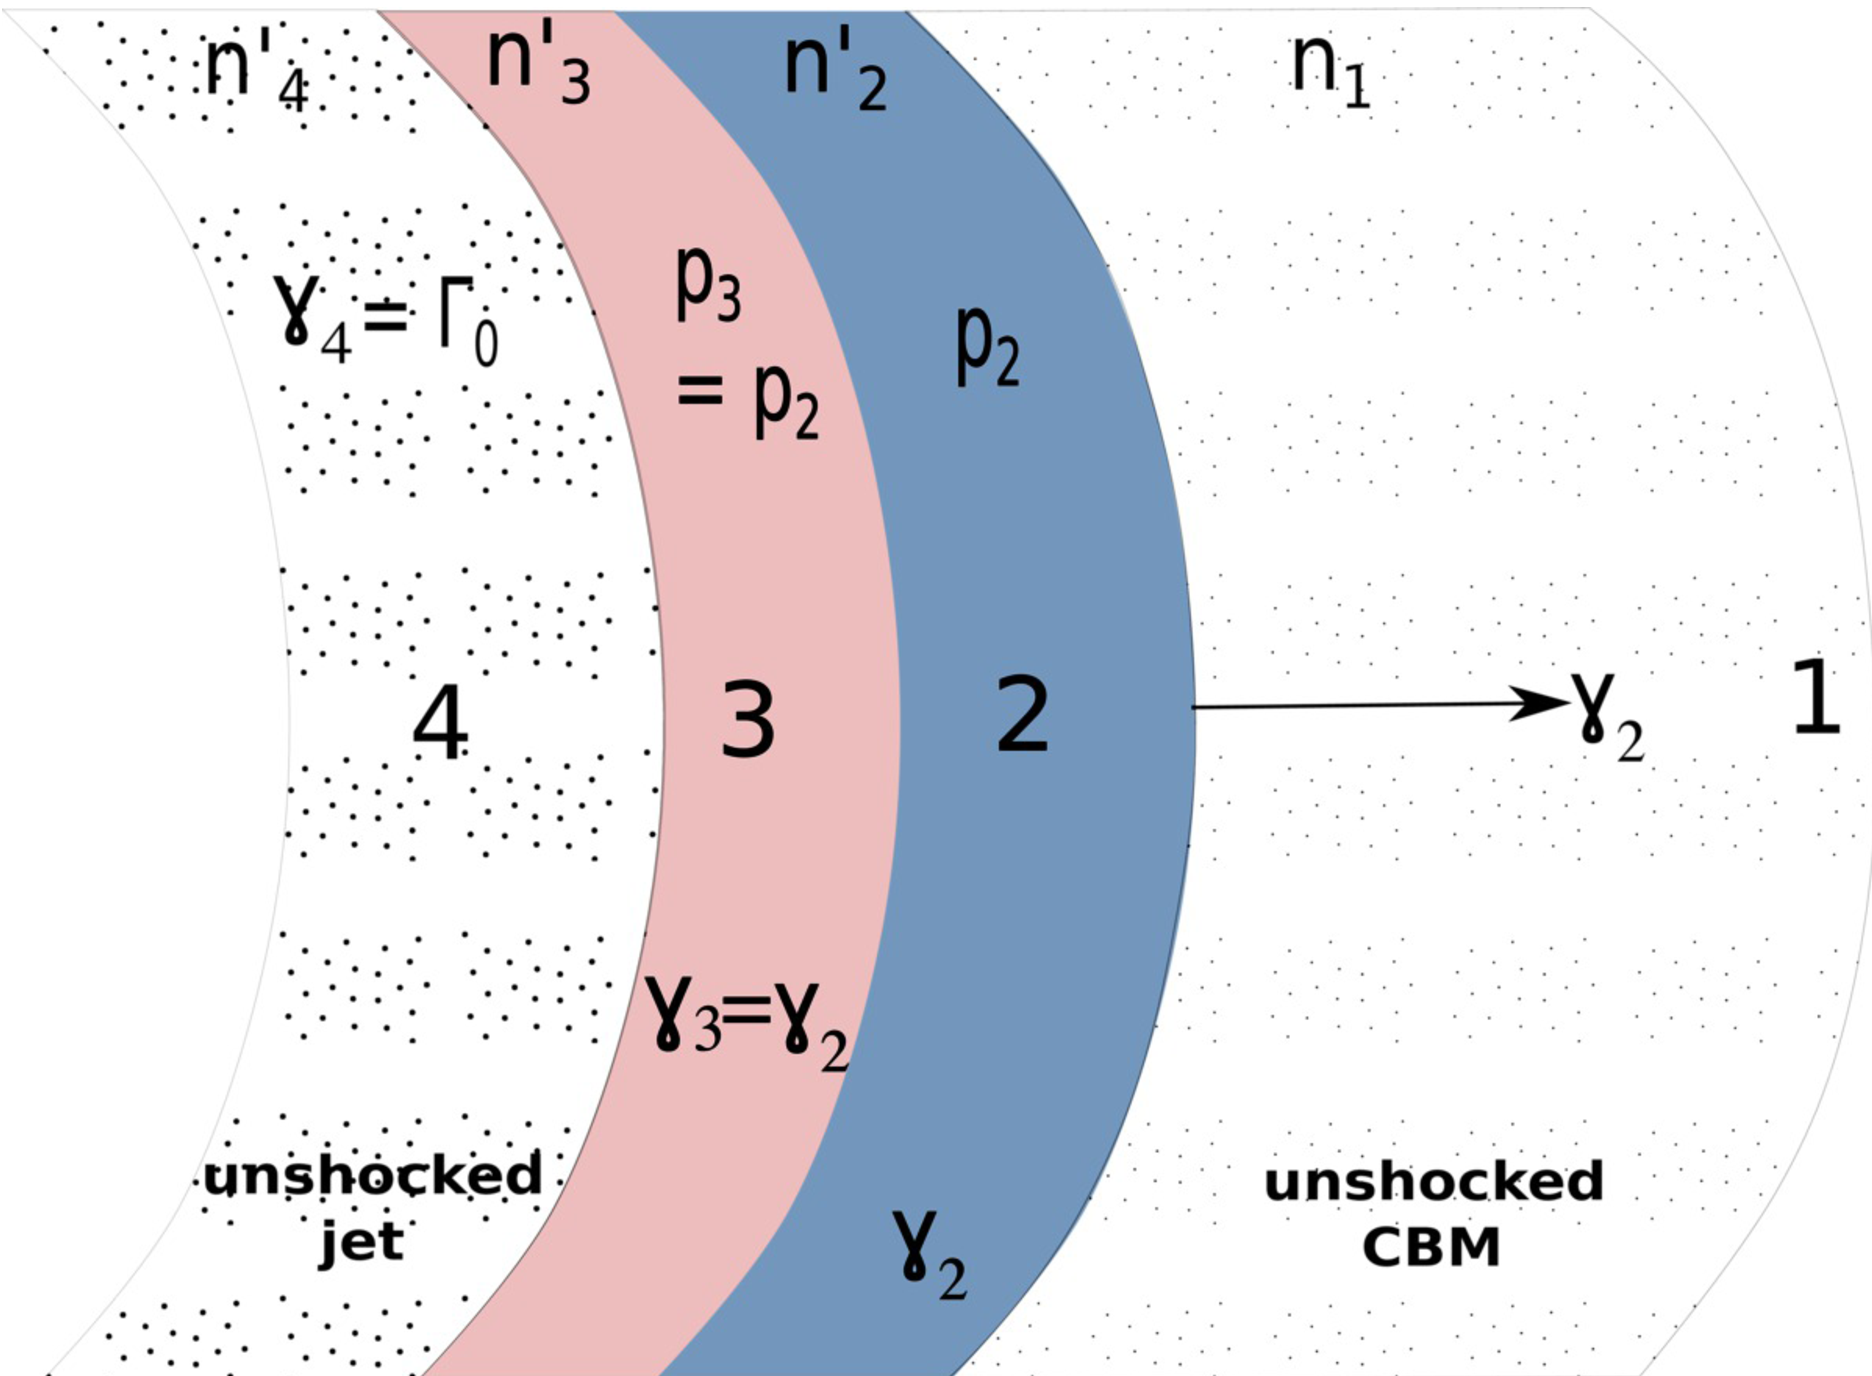
\includegraphics[width=0.45\textwidth]{Fig_8_KZ.pdf}
    \caption{
        This is a schematic sketch of a pair of shocks produced when a relativistic
        jet from a \ac{GRB} collides with the \ac{CBM}, as viewed from the
        rest frame of unshocked \ac{CBM}. Regions 2 \& 3 represent shocked \ac{CBM} and \ac{GRB}
        jet respectively. They move together with the same \ac{LF} ($\gamma_2$, as viewed
        by a stationary observer in the unshocked \ac{CBM}), and have the same pressure but
        different densities.
        (Adapted from \citet{Kumar:2014upa}, Fig.~8)
    }
    \label{fig:aafg:theory:sr8}
\end{figure*}

Here, in Fig.~\ref{fig:aafg:theory:sr8} \red{same as in Nava picture that you should put} the $2$ and $1$ subscripts stand for downstream and upstream respectively, $e'$ is the internal energy density, $n'$ is the proton number density, (both in the local fluid rest frame), $\gamma_{21}$ is the relative \ac{LF} of plasma in region $2$ with respect to the region $1$, $\gamma_{1s}$ is the relative \ac{LF} of plasma in region $1$ with respect to the shock front and $\hat{\gamma}$ is the adiabatic index of the fluid.

For $\Gamma\gg1$ that usually describes early stage of the \ac{GRB} afterglow \cite{Piran:1999kx}, the $\hat{\gamma}=4/3$ \red{recall that in subrelativistc it is $5/3$}
%% ---
Then, $n_2'/n_1' = 3 ((4/3)\gamma_{21} + 1) = 4\gamma_{21} + 3 \approx 4\gamma_{21}$ which implies that the downstream plasma is compressed with compression ratio $4\gamma_{21}$.
Similarly, approximating, the conservation equation $\frac{e_2'}{n_2'} \approx \gamma_{21} m_p c^2$ and the last equation can be simplifed to $\gamma_{1s} \approx \sqrt{2} \gamma_{21}$, which implies that the shock front travels faster then the downstream fluid.

Next, consider the self-similar deceleration phase of the blast wave in the constant density \ac{CBM}. There, the energy consirvation reads 

\begin{equation}
E = \frac{4 \pi }{3 } R^3 n m_p c^2 \Gamma^2 = \text{ const}
\end{equation}

where $\Gamma = \gamma_{21}$ is the \ac{LF} of the blastwave with respect to the unshocked medium, $R$ is the radius of the blast wave (from \ac{CoE}).
Note, that in the comoving frame the average proton thermal energy is $m_p c^2 \Gamma$. 
In the lab frame it is $m_p c^2 \Gamma^2$. 
Overall, we observe that $\Gamma^2 R^3 = \text{ const}$ or 

\begin{equation}
\Gamma \propto R^{-3/2}
\end{equation}

Now, consider the elapsed time in the observer frame. 
As both the blast wave and emitted photons are moving in the same direction with the speed difference of $\sim 1/2 \Gamma^2$, 

\begin{equation}
t_{obs} \sim \frac{R}{2\Gamma^2 c} \propto R^4 \propto \Gamma^{-8/3}
\end{equation}

and 

\begin{equation}
\Gamma \propto R^{-3/2} \propto t_{obs}^{-3/8}, \hspace{3mm} R\propto t_{obs}^{1/4}
\end{equation}

%%______________________________________
%% on the non-uniform CBM

Next, we consider \red{power-law stratified density profile}, 

\begin{equation}
n = n_0 \Big(\frac{R}{R_0}\Big)^{-k}
\end{equation}

and obtain similar scaling relations.
\red{I do not really need this. I can go directly to Peer model and Nava model}

\begin{equation}
E = \int n_0 \Big( \frac{R}{R_0} \Big)^{-k} m_p c^2 \Gamma^2  4\pi R^2 dR = \text{ const}
\end{equation}

where $R^{3-k} \Gamma^2 \text{ const}$. 

After some derivation 

\begin{equation}
\Gamma\propto R^{(k-3)/2}\propto t_{obs}^{(k-3)/(8-2k)}
\end{equation}

And if $k=0$, the previously derived relation for constant density CBM follows.

A particularly useful case is the \ac{CBM} filled with a free wind with constant mass loss rate $\dot{M}$ and wind speed $\upsilon_w$, that gives $\dot{M}=4\pi R^2 n \upsilon_w = \text{ const}$, or $n\propto R^{-k}$, \ie, the case of $k=2$ with $\Gamma\propto R^{-1/2}\propto t_{obs}^{-1/4}$.

%%_______________________________________
%% On the energy injection

Now consider the case where the energy of the blast wave is continuously increasing. A possible physical scenario here is a long-lasting Poynting-flux dominated jet, feeding the fireball \gray{and suppressing the reverse shock}. 
Then the energy of the outflow from the central engine has to be included into the energy equation of the blast wave

\begin{equation}
E_{tot} = E_0 + E_{inj}
\end{equation}

Consider a central engine with time dependent luminocity  $L(t) = L_0 (t_{obs}/t_0)^{-q}$. Then the energy equation reads

\begin{equation}
E_{tot} = E_0 + E_{inj} = E_0 + \int_{0}^{t_{obs}} L(t)dt = E_0 + \frac{L_0 t_0^q}{1-q}t_{obs}^{1-q}
\end{equation}

where $E_0$ is the initial energy of the blast wave and $E_{inj}$ is the injected energy into the blast wave from the central engine.

Consider the case when energy injection increases with time noticeably, $q<1$.

Then, when $E_{inj} \gg E_0$ for $q<1$, the blast wave scaling 

\begin{equation}
E_{tot} \sim E_{inj} \propto t_{obs}^{1-q}.
\end{equation}

and for the constant density \ac{CBM}, $\Gamma^2 R^3 \propto t_{obs}^{1-q}$ which eventually leads to $\Gamma\propto R^{-(2+q)/(4-2q)}\propto t_{obs}^{-(2+q)/8}$.

And it is easy to see that if $q\rightarrow 1$, the 'no injection' case is resored.

%%____________________________________
%% Lorentz factor stratification of the ejecta as the Energy injection

The energy can be added to the blast wave in a form of velocity stratified ejecta, when the wave decelerates, \eg,

\begin{equation}
E\propto \gamma^{1-s}\propto\Gamma^{1-s}
\end{equation}

where $\gamma$ is the \ac{LF} of the ejecta and $\Gamma$ is the \ac{LF} of the blast wave.
Here the effects of the reverse shock can also be neglected as energy injection comes when $\Gamma\sim\gamma$ \red{[How does this work in the Peer/Nava model?]}

This method is equivalent to the long-lived central engine with time dependent luminosity (at least for the dynamics of the blast wave), and the coefficient $s$ can be expressed in terms of $q$ \cite{Zhang:2005fa}. 

For a uniform density \ac{CBM} the scaling relation reads

\begin{equation}
\Gamma\propto R^{-3/(1+s)}\propto t_{obs}^{-3/(7+s)}, \hspace{3mm} R\propto t_{obs}^{(1+s)/(7+s)}
\end{equation}

which then gives $s = (10-7q)/(2+q)$ and $q=(10-2s)/(7+s)$

\red{The question is, can I add L(t) to the dE/dr of the Nava model and it is all?..}



\subsection{Afterglow synchrotron spectrum and \ac{LC}}

\red{Note that here the electron distribution function is implicitly assumed such that $dn/d\gamma$ peaks at $\gamma_m$ and for $\gamma>\gamma_m$, the $dn/d\gamma\propto\gamma^{-p}$,and for $\gamma<\gamma_m$, the distribution is uncertain. It could be thermal}

\cite{Sari:1997qe} has shown that the multi-segment broken power law function can \gray{sufficiently well} describe the instantaneous afterglow spectrum. The spectrum consists of three characteristic frequencies: the \red{typical synchrotron frequency of the accelerated electrons with the minimum \ac{LF}} $\nu_m$, the cooling frequency $\nu_c$ and the synchrotron self-absorption frequency $\nu_a$.
The latter is usually the smallest one in the afterglow phase (at least for a few months \gray{but it depends on the \ac{CBM} density}).
Depending on the order of $\nu_m$ and $\nu_c$ the spectrum falls into two broad categories. The \textit{slow cooling} case, when $\nu_m < \nu_c$ and a \textit{fast cooling} case when $\nu_m > \nu_c$. The scaling relations for these regimes are \cite{Sari:1997qe}

\begin{equation}
f_{\nu} = 
\begin{cases}
f_{\nu,\max}\Big(\frac{\nu_a}{\nu_m}\Big)^{1/3}\Big(\frac{\nu}{\nu_a}\Big)^2 & \text{ if } \nu < \nu_a \\
f_{\nu,\max}\Big(\frac{\nu}{\nu_m}\Big)^{1/3} & \text{ if } \nu_a < \nu < \nu_m \\
f_{\nu,\max}\Big(\frac{\nu}{\nu_m}\Big)^{-(p-1)/2} & \text{ if } \nu_m < \nu < \nu_c \\
f_{\nu,\max}\Big(\frac{\nu_c}{\nu_m}\Big)^{-(p-1)/2}\Big(\frac{\nu}{\nu_c}\Big)^{-p/2} & \text{ if } \nu > \nu_c \\
\end{cases}
\end{equation}

for the \textit{slow cooling} case and 

\begin{equation}
f_{\nu} = 
\begin{cases}
f_{\nu,\max}\Big(\frac{\nu_a}{\nu_c}\Big)^{1/3}\Big(\frac{\nu}{\nu_a}\Big)^2 & \text{ if } \nu < \nu_a \\
f_{\nu,\max}\Big(\frac{\nu}{\nu_c}\Big)^{1/3} & \text{ if } \nu_a < \nu < \nu_c \\
f_{\nu,\max}\Big(\frac{\nu}{\nu_c}\Big)^{-1/2} & \text{ if } \nu_c < \nu < \nu_c \\
f_{\nu,\max}\Big(\frac{\nu_m}{\nu_c}\Big)^{-1/2}\Big(\frac{\nu}{\nu_c}\Big)^{-p/2} & \text{ if } \nu > \nu_m \\
\end{cases}
\end{equation}

from the \textit{fast cooling} case. 

Here $f_{\nu;max}$ is the flux density which $f_{\nu}(\nu_m)$ for the slow cooling case and $f_{\nu}(\nu_{c})$ for the fast cooling. \red{this is the answer  I was looking for}. 

Note that in this formalism, the scaling relations, spectrum, does not depend on the blast wave dynamics. Only the peak flux $f_{\nu,\max}$, and the characteristic frequencies $\nu_a$, $\nu_c$, $\nu_m$ do. 

The characteristic frequencies $\nu_m$, $\nu_c$ can be calculated from the synchrotron frequency formula (see previous sections)

\begin{equation}
\nu = \frac{3}{4\pi}\gamma^2\frac{qB'}{m_e c}
\end{equation}

where $\gamma$ is $\gamma_{m}$ or $\gamma_c$. 

The minimum \ac{LF} in the shock heated plasma with a given electron distribution (power law) is

\begin{equation}
\gamma_m = g(p) \varepsilon_e (\Gamma - 1) \frac{m_p}{m_e}\frac{n_p}{n_e},
\end{equation}

where $\Gamma$ is the \ac{LF} of the blast wave, $\varepsilon_e$ is the fraction of energy density of the shocked fluid given to electrons, $n_p$ and $n_e$ are the number densities of the protons and electrons respectively, and $g(p)$ is the dimensionless factor

\begin{equation}
g(p) \approx 
\begin{cases}
\frac{p-2}{p-1} & \text{ if } p>2 \\
\ln^{-1}(\gamma_M/\gamma_m), & \text{ if } p = 2
\end{cases}
\end{equation}

where $\gamma_M$ is the maximum \ac{LF} of electrons.

\gray{
    the $gamma_min$ and its dependency on $g(p)$ seems to come from equating the integral of the electron distribution function for $\gamma>\gamma_min$ to the total energy density of the shocked fluid, \ie, $4\Gamma (\Gamma - 1) n_p m_p c^2$ times the fraction of this energy available, $\varepsilon_e$. 
    [If this is the case, maybe I can compute it numerically?..]
}

The cooling \ac{LF} of electrons is derived based on the cooling timescale (see previous sections)

\begin{equation}
\gamma_c = \frac{6\pi m_e c}{\sigma_T t' B^{'2} (1 + Y)}
\end{equation}

where $Y = u_{syn}/u_{B}$ is the \ac{SSC} parameter, which depends whether the photon-electron scattering is in Klein-Nishina limit (\ie, if photon energy exceeds $m_e c^2$),
the $u_{syn}$ is the synchrotron photon energy density and $u_B$ is the magnetic energy density.

The \ac{SSA} frequncy can be obtained by equating the black-body flux corresponding to the temperature of electrons with characteristic frequency $\nu_a$ to the emerging flux at $\nu_a$, 

\begin{equation}
I_{\nu}^{syn}(\nu_a) = I_{\nu}^{bb}(\nu_a) \approx 2 k_B T \frac{\nu_a^2}{c^2}
\end{equation}

where 

\begin{equation}
k_B T \approx \max[\gamma_a,\min(\gamma_c,\gamma_m)] m_e c ^2 /3
\end{equation}

where $\gamma_a$ corresponds to $\nu_a'$ as $\gamma_a = (4\pi m_e c \nu_a' / 3qB')^{1/2}$.

Assuming that a fraction, $\varepsilon_B$, of the energy density of the shocked \ac{CBM} goes into the magnetic filed energy density, the magnetic field strength reads 

\begin{equation}
B' \approx [32 \pi m_p c^2 \varepsilon_B n_p (\Gamma - 1)\Gamma]^{1/2}
\end{equation}

Next the scaling for the $\nu_m$, $\nu_c$ and $\nu_a$ are provided based on the shock dynamics in different \ac{CBM}. 
For instance, for the case of constant density medium see \citet{Granot:2001ge,Gao:2013mia} and for wind-like \ac{CBM}.. 

The maximum of the specific flux $f_{\nu,\max}$ is (see previous section)

\begin{equation}
f_{\nu;\max} = \frac{(1+z)L'_{\nu'}\Gamma}{4\pi D_L^2} \approx (1+z)\frac{N_{tot}P_{\nu;\max}' \Gamma}{4\pi D_{L}^2}
\end{equation}

where $L'_{\nu'}$ is the specific luminocity in the jet comoving frame, $N_{tot}$ is the total number of electrons that contribute to radiation at frequency $\nu$

\begin{equation}
P_{\nu',\max}' = \approx \frac{\sqrt{3} q^3 B'}{m_e c^2}
\end{equation}

is the power radiated per unit frequency for one electron at the peak of the spectrum, or in other words it is the specific power for electron with thermal \ac{LF} $\gamma\approx\min(\gamma_c,\gamma_{min})$ and $z$ is the Redshift of the burst and $D_L$ is the luminosity distance to it.

Note that for a constant density \ac{CBM}, the $F_{\nu,\max}$ is time independent as $F_{\nu,\max}\propto R^3\Gamma^2\propto E_{tot}$ total energy of the blast wave (which is constant for an adiabatic external shock). For the constant density \ac{CBM} and wind-like \ac{CBM} see full expression for the peak specific flux \citep{Granot:2001ge,Yost:2003mw} 

Note more that for $\nu>\max[\nu_m,\nu_c]$, the observed specific flux \citep{Kumar:1999eu,Freedman:1999mp} is independent on the \ac{CBM} density and its stratification and depends weakly on $\varepsilon_B$, 

\begin{equation}
f_{\nu} \propto E^{(p+2)/4} \varepsilon_e^{p-1}\varepsilon_B^{(p-2)/4}t_{obs}^{-(3p-2)/4}\nu^{-p/4}
\end{equation}

This is of particular importance for high energy emission from \ac{GRB}.



\subsection{Reverse shock}
\red{This is very short section, not very clear in the source}

If the \ac{GRB}-ejecta magnetization is not important dynamically $\sigma \ll 1$, (where magnetization parameter $\sigma B^{'2}/(4\pi n_p' m_p c^2)$), the \ac{RS} is traversing the ejecta during the early afterglow. \red{The \ac{RS} decelerates the ejecta}

The \ac{RS}-\ac{FS} system can be represented via $4$ regions (see Fig.~\ref{fig:aafg:theory:sr8} or a Fig from Nava) that consists of: $1.$ unshocked medium, $2.$ the shocked medium, (separated from the reion $1$ by the forward shock front), $3.$ the shocked ejecta and $4.$ the unshocked ejecta, with reverse shock front separating $3$ and $4.$.

The shock fronts $1-2$ and $3-4$ are surfaces of contact density-discontinuity.

%% observed
The RS heated ejecta was observed first in the case of \ac{GRB} 990123 as an optical flash while the burst was still active \citep{Akerlof:1999aa,Sari:1999a,Meszaros:1999gb}.

%% deriviation of RS 
\red{Here Nava paper would be much better}
The derivation of the \ac{FS}-\ac{RS} dynamics is based on the pressure equilibrium across the contact discontinuity surfaces (separating regions $2$ and $3$ \red{note that these are not shock fronts}). 
Consider and unmagnetized \ac{GRB} jet. 
%%% --- 
Introduce $\gamma_{12}$ and $\gamma_{34}$, \ac{LF}s of the \ac{FS} (\ac{RS}) heated \ac{CBM} (GRB-ejecta) with respect to the unshocked \ac{CBM} (\ac{GRB}-ejecta). The shocked fluid pressure in regions $2$ and $3$ is $4\gamma_{21}^2 n_1$ and $4\gamma_{34}^2 n_4'$ respectively, where $n_1'$ and $n_4'$ are the densities of the unshocked medium in the \textit{local} comoving frame.
Note that the \ac{LF} of the unshocked ejecta ($4$) with respect to the unshocked \ac{CBM} ($1$), \eg, $\gamma_{41}=\Gamma_0=2\gamma_{21}\gamma_{34}$, where the latter \ac{RHS} is derived based on the addition of $4$-velocities. Then, together with pressure equilibrium across the discontinuity surface \gray{presumably $2$ and $3$} it yields

\begin{equation}
\gamma_{34} \approx (n_1/4n_4')^{1/4}\Gamma_0^{1/2} \text{ and } \gamma_{21} \approx (n_4'/4n_1)^{1/4}\Gamma_0^{1/2}.
\end{equation}

Note, that here the fact that the \ac{RS} and \ac{FS} are relativistc is assumed. \red{For non-relativistic \ac{RS} the derivation is defferent}.

Note that the $\gamma_{31}$, the \ac{LF} of the shocked jet with respect to the \ac{CBM} is equal to $\gamma_{21}$, as both shocks are moving with the space velocity. 

Now, obtained $\gamma_{ij}$ allows to study the thermodynamic properites of the \ac{FS}/\ac{RS} system. For \red{full} derivation of these formalism see \citep{Sari:1995}.

%% Radiation into?
TO simplify the calculations of rhe radiation from the RS, the finite size of the GRB-jet and constant lorentz factor of the ejecta are usually assumed. This size corresponds to the finite duration of the GRB.
\gray{The velocity stratified ejecta howere is possible and induce interesting features in the \ac{RS} lightcurve \citep{Rees:1997nx,Sari:2000ks,Uhm:2007nc,Genet:2007nb,Uhm:2012,Uhm:2014qta}
} 
Then, adiabatic coolding of electrons and decline in magnetic field strength (after the RS reaches the back of the ejecta) results in a steep fall of the RS radiation $\sim t^{-2}$ \citep{Sari:1999b}. 

%% back to the dynamics
The \ac{FS}/\ac{RS} shock dynamics ultimately depends on the width of the ejecta, \citep{Sari:1995}

\begin{equation}
\xi = (l/\Delta)^{1/2}\Gamma_0^{-4/3},
\end{equation}

where $l$ is the Sedov radius \red{the radius at which the rest mass energy of the swept up \ac{CBM} by the blast wave is equal to the initial energy of the \ac{GRB}}. 
$\Delta$ is the thickness of the \ac{GRB}-ejecta in lab frame, with $T$ being the duration of the burst in the \ac{CoE} frame. 
Based on $\xi$ the \ac{GRB} ejecta is considered to be a "thin shell", if $\xi > 1$ or a "thin shell" if $\Xi < 1$, and the shock dynamics is different in these two cases.

%% Literature
See \citet{Kobayashi:2000af} for the discussion of the \ac{FS}/\ac{RS} dynamics and radition emitted discussion.
Additionally see \citet{Kobayashi:2003zk,Kobayashi:2002uw,Zhang:2003wj,Kumar:2003fy,Wu:2003,Gao:2013mia} for the \ac{FS}/\ac{RS} emisison properties.

Additionally, see \citet{Zhang:2004ie,Mimica:2008up,Narayan:2011} for the shock solution for a jet with arbitrary magnetization $\sigma$ and the work of \citet{Fan et al. (2004)} for the case of $\sigma < 1$. 

The ration of microphysical parameters in FS and RS, as well as their lorentz factors determine how important is the RS emission. 
\citep{(Kobayashi and Zhang, 2003b; Zhang et al., 2003a; Nakar and Piran, 2004)}
If the emission from FS and RS can be separated in the afterglow data, then the RS radiation provides one of the few hints into the GRB-ejecta composition 
\citep{McMahon et al. (2006); Nakar and Piran (2004)}

With respect to the ratio FS/RS different observational features are present \citep{(Zhang et al., 2003a; Jin and Fan, 2007)}.

\textit{Type I: re-brightening}. Assuming common values for $\varepsilon_e=0.1$ and $\varepsilon_B=0.01$, for FS and RS, the optical lightcurve exhibits a double peak structure, with the first peak dominated by RS and second by FS. It was observed \citep{Kobayashi and Zhang, 2003b; Shao and Dai, 2005}. 

\textit{Type II: flattening}. If the RS has stronger magnetic field then FS, and the magnetisation parameter for region $4$ is small enough for not to supress the RS, the emission from the RS dominates the early afterglow, peaking when the RS reaches the end of the GRB-ejecta, after which it decays $\propto t^{-2}$ (\citep{Meszaros and Rees, 1999; Sari and Piran, 1999b}). At some point the decay takes over, cahnging the decay behaviour to $\propto t^{-1}$. This has observational support \citep{(Fox et al., 2003; Li et al., 2003; Zhang et al., 2003a; Kumar and Panaitescu, 2003; Gomboc et al., 2008}

\textit{Type III: no RS component}
Many observed optical afterglow shows a smooth hump with a post-decay slope consistent with FS emission and nos signatures of RS \citep{Molinari et al., 2007; Ryko et al., 2009; Liang et al., 2010}.
A possible explanation is that Poynting flux dominates the GRB-jet and supresses the RS 
\citep{Zhang and Kobayashi, 2005; Mimica et al., 2009}.



\subsection{Jet Break}

\red{The convention is to call the jet with uniform structure a top-hat jet...}

Here we consider effects of a finite jet angle on the observed lightcurve.

The observations of GRB afterglow, specifically, the observed achromatic break, suggested that GRB-jet is collimated. The achromatic break in the lightcurve, usually referred to as "jet break", has in its origin two main effects \cite{Rhoads, 1999; Sari et al., 1999}. 

First, is a pure geometric effect, called "edge" effect \cite{(e.g.Meszaros and Rees, 1999; Panaitescu and Meszaros, 1999; Rhoads, 1999; Sari et al., 1999}. Specifically, for a GRB-jet with openning angle $\theta_j$, the observer sees only the radiation coming from within the $1/\Gamma$ cone due to relativistic beaming. Thus, if $\Gamma > 1/\theta_j$, the radiation from only a fraction of the jet an observer sees. Such "pre-jet-break" lightcurve appears indistinguishable from a lightcurve from isotropic fireball (as in any case only a cone of $1/\Gamma$ is visible). 
As the jet decelerates, however, the $1/\Gamma$ cone grows and when the photon beaming angle equates the openning angle of the jet-cone, the lightcurve shows a 'Jet break", after which the observed radiation starts to fall off more steely then before the "jet break". 
Note, the "edge effect" is geometrical and special relativistic, effect. The jet dynamics does not change as well as the temporal behavior of characteristic frequencies. Only the observed temporal behavior of lightcurves. 
In order to account for this effect, the factor $\theta^2_j/(1/\Gamma)^2 \propto \Gamma^2$ is introduced.
In the case of uniform CBM, where $\Gamma\propto t^{-3/8}$, the post-jet-break lightcurve falls off faster by a factor $\Gamma^2\propto t^{-3/4}$.

Note, that the effect of jet-break smears out by the integration over equal-time-arrival surface \cite{Kumar and Panaitescu, 2000b; Piran, 2000; Granot and Piran, 2012}.

%% LATERAL EXPANSION

Next, consider the jet sideways (lateral) expansion.
It was shown that the the jet lateral expansion, (when the sound waves cross it) occures apporximatelly at a time when the "edge effect" becomes important \cite{Rhoads (1999) and Sari et al. (1999)}.
%% See page 37 for original text. It is very messy.
Consider a sideways expansion speed of the jet in comoving frame. For relativistic plasma it is $c/\sqrt{3}$. Then, the jet openning angle grows as $\theta_j\sim\Gamma_{(ij)k}^{-1}$, as a result of time dialation and transverse speed being $\sim c$. Thus, in the jet comoving frame, the elapsed time is $1/\Gamma$ of the elapsed time in the lab frame. In its oww, rest frame the the transverse size of the jet epanding with $\sim$ is $\sim R/\Gamma$, while in the lab frame the transverse speed is $\upsilon_{\theta}\sim c/\Gamma$.
From the momentum equation if follows hwoever that for a relativisic plasma $\partial(\rho\Gamma^2\upsilon_{\theta})/\partial t \sim r^{-1}\partial p / \partial\theta$, which leads to $\upsilon_{\theta}\sim c/(\Gamma^2\theta_j)$.
See \cite{Kumar and Granot (2003)} \cite{Granot and Piran (2012)} for the detailed discussion.
\red{Note that in the 'code' we use the Granot and Piran (2012) model as well.}

Analytically it can be shown that, after the jet-break the jet $R$ increase slows down \textit{e.g.,}
\cite{Rhoads (1999); Sari et al.(1999); Piran (2000); Granot and Piran (2012)}.
A simple scaling relations for $\nu_m$, $\nu_c$ and $F_{\nu;max}$ as well as $f_{\nu}=f_{\nu}(\nu, t_{obs}, p)$ can be obtained.
Importantly, the flux at a frequncy taht lies above the $\min(\nu_c,\nu_m)$decays faster with the jet lateral expansion (compare to the "edge effect" alone).

It was shown that the sideways expansion becomes important only after the $\Gamma$ falls below $2$ \cite{(Granot et al., 2001; Kumar and Granot, 2003; Cannizzo et al., 2004; Zhang and MacFadyen, 2009; De Colle et al., 2012; Granot and Piran, 2012; van Eerten and MacFadyen, 2012; van Eerten et al., 2012)}
\red{Really??}

However, the observed lightcurve depends on the observer's vewving angle \textit{e.g.,} \cite{Zhang et al., 2014b; Ryan et al., 2014).}.

% STRUCTURED JET

It is expected that the GRB jet has an angular structure with luminosity per solid angle and Lorentz factors depending on the the angle.
Commonly assumed structure times include the dependence of jet properties on the angle as a power-law function
\cite{(Meszaros et al., 1998; Rossi et al., 2002; Zhang and Meszaros, 2002b)} 
and Gaussian distribution 
\cite{(Zhang and Meszaros, 2002b; Kumar and Granot, 2003; Zhang et al., 2004a).}
The structure of the jet becomes very importnat when the jet is observed off-axis, while for an on-axis observer, the afterglow has a steeper decay in coamparsion to a simple "top-hat" jet \cite{Meszaros et al., 1998; Dai and Gou, 2001; Panaitescu, 2005}
For an off-axis observer, seeing the power-law jet, the "jet break" time depends on the viewing angle $\theta_{\upsilon}$ (contrary to the $\theta_j$ jet openning angle as in top-hat jet)
\cite{Zhang and Meszaros, 2002b; Rossi et al., 2002; Kumar and Granot, 2003; Granot and Kumar, 2003}.
For an off-axis observer, seeing the gaussian get, the observed lightcurve depends on whether the $\theta_{\upsilon}$ falls within the gaussian cone. If yes, then the observed emission is similar to the "top-hat" jet. If no, then it is similar to the power-law jet.
\cite{Kumar and Granot, 2003; Granot and Kumar, 2003}

Importantly, that structured jet allows to introduce the so called "quasi-universal" GRB, \cite{(Rossi et al., 2002; Zhang and Meszaros, 2002b; Zhang et al., 2004a)}. The GRB jets are considered to the similar, appear only different to the observer due to different viewing angles (see \textit{e.g.,} \cite{Zhang and Meszaros, 2002b}).
See the \cite{(Zhang and Meszaros, 2002b; Rossi et al., 2002} for the similarities in the luminocity functions of structured jets. 
It was however shown that quasi-universal jet does well agree with observations \cite{(Nakar et al., 2004}. But with more free parameters, it might be more consistent with observational constraints \cite{(Lloyd-Ronning et al., 2004; Zhang et al., 2004a; Dai and Zhang, 2005)}

%% TWO compnent Jet Model

As a subcategory of structured jets, a two-component model has been widely consdiered. Such model consits of a collimated energetic get with high $L_{\gamma,iso}$ and $\Gamma$, surrounded by a wider and slower \gray{cocoon}. 
Such model can account for certain observational features, \textit{e.g.,} for early jet break and subsequent rebrightening
\cite{Huang et al., 2004; Peng et al., 2005; Wu et al., 2005}.
Particular application of the model GRB 030329 \cite{(Berger et al., 2003b)} and GRB 080319B \cite{(Racusin et al., 2008).}.
Such model is particularly favioured for the collaspar scenario, where the narrow, highly relativist jet emerges from a star, in addition to the wide, less relativistic "cocoon" around it \cite{Ramirez-Ruiz et al., 2002; Zhang et al., 2004b}. 

%%

Another example of a structured jet is a "patchy" jet, where numerous "mini-jets" within a broad jet cone are the source of the bright emission \cite{Kumar and Piran, 2000a; Yamazaki et al., 2004b}.
Such structure can occure when there are non-uniform shells present.
The patches of the accelerated emission regions can be present within relativisitc outflowed due to magnetic reconnections or turbulence in a magnetically domianted jets \cite{Luticov and Blandford, 2003; Narayan and Kumar, 2009; Kumar and Narayan, 2009; Lazar et al., 2009; Zhang and Yan, 2011; Zhang and Zhang, 2014}

%%

\textit{Orphan afteglows}

The orphan afterglow is the afterglow detected without prompt $\gamma$-ray emission. This can occur if the line of sight to the observer lies outside the cone of relativistically beamed photons from the jet. However, as the Doppler beaming factor inceases (as the $1/\Gamma$ cone widens), and the observed emission rises. It peaks when the line of sight crosses the $1/\Gamma$ cone. After that, the lightcurve behaves in accordince with the post-jet-break afterglow \cite{Granot et al., 2002}.
\textit{dirty fireball} is one of the scenarios where the ophan afterglow is possible, as its low $\Gamma$ prevents the promt energetic emission from arising \cite{Huang et al., 2002).}. 
The detection of such afterglows however is very challenging.

%%
%%
%%

\subsection{Other Effects}

The effects of radiative losses on the blastwave dynamics, and afterglow lightcurves
\cite{e.g. Rees and Meszaros, 1998; Dermer et al., 1999; Meszaros and Rees, 1999; Huang et al., 1999; Bottcher and Dermer, 2000; Nava et al., 2013} and \red{are not discussed} here.

%%

\subsubsection{Naked afterglow and high-latitude effect}

At a certain distance from the CoE, a blastwave may encounter a void. But even though, the acceleration of new electrons (and their subsequent adiabatic cooling) stops, the observed emission does not shuts down instantaneously. The reason is the lorentz beeming. Photons from angles larger then $1/\Gamma$ with respect to the line of sight continue to contribute to the observed flux for some time. This is so-called "high latitude" radiation. It has a signature $f_{\nu}\propto t^{-\alpha}\nu^{-\beta}$, where $\alpha= \beta + 2$. See \cite{Fenimore et al. (1996); Kumar and Panaitescu (2000a); Dermer (2004)}.
This effect is believed to the responsible for steep delcining X-ray lightcurves of some GRBs \cite{Zhang et al., 2006}.

%%

\subsubsection{Energy injection}

In addition to the continous energy injection (from a central engine or outflow), discussed above, there is also a possibility of a dsecrete energy injection. This can occure if fast shells of ejecta catch up with the blast wave. Interaction of such shell with blast wave can be described in terms of five (six) different regions separated by three shocks \cite{(Kumar and Piran, 2000b)} (\cite{(Zhang and Meszaros, 2002c)}). 
Such energy injection leads to a diverse range of features in afterglow, as abrupt optical rebrightening. \cite{(e.g. Nardini et al., 2011} \cite{Zhang and Meszaros, 2002c}

%%

\subsubsection{Density Bumps}

It was suggested that the sudden incease in density of the curcumburst medium may introduce bump features in lightcurves \cite{Dai and Lu, 2002; Lazzati et al., 2002; Dai and Wu, 2003; Pe'er and Wijers, 2006}. However, numerical simulations \cite{Nakar et al., 2003; Nakar and Granot, 2007; Uhm and Beloborodov, 2007; Uhm and Zhang, 2014a; Geng et al., 2014)} showed that the re-brightening feature should appear very smooth dues to the integration over the (relativistc) equal-arrival-time surfaces, which manifests that the observed emission at any given time is given by the blastwave at different latitudes and emission times.
Moreover, for the high energy bands (above $X$-ray, where $\nu>\nu_c$), the \red{the observed flux is independent of the ambient density} \cite{Kumar, 2000; Freedman and Waxman, 2001}.

%%

\subsubsection{Synchrotron self-Compton}

The Synchrotron self-Compton emission allows electrons to cool more efficiently, reducing the corresponding frequency by $(1+Y)^2$ \cite{(e.g.Wei and Lu, 1998; Panaitescu and Kumar, 2000; Sari and Esin, 2001)}; where $Y = u_{sun}=u_{B}$ is the ratio of synchrotron photon energy density and magnetic field energy density. 
It also modifies the spectrum, adding a high energy component that in principle could dominate the GeV band and appear in late $X$-ray lightcurve if the ambient density is sufficiently large engough
\cite{Meszaros and Rees, 1993; Meszaros et al., 1994; Sari and Esin, 2001; Zhang and Meszaros, 2001b}.
Additionally, if the IC cooling occure in the Klein-Nishina regime, the index of synchrotron spectrum could be less steep \cite{e.g. Derishev et al., 2001; Nakar et al., 2009; Daigne et al., 2011; Barniol Duran et al., 2012}. 
While for most GRBs the GeV emission can be explaiend by the synchrotron mechanism operating in the forward shock alone, \cite{(e.g. Kumar and Barniol Duran, 2009, 2010)}, for certain cases, \textit{e.g.,} GRB 130427A \cite{Ackermann et al., 2014} a possible IC component might be required to explain the observations \cite{e.g. Fan et al., 2013a; Liu et al., 2013}.

%%

\subsubsection{Hard electron spectrum}

The effects of energy injection on the afterglow lightcurve, \textit{shallow slope}, cam be mimicked by a electron spectrum with $p\in(1,2)$. In this regime, the minimum electron LF depends on the maximum as 

\begin{equation}
\gamma_m = \Bigg( \frac{2-p}{p-1} \frac{m_p}{m_e} \varepsilon_e \Gamma \gamma_M^{p-2} \Bigg)^{1/(p-1)}
\end{equation}

\cite{cf. (Dai and Cheng, 2001; Bhattacharya, 2001; Resmi and Bhattacharya, 2008}.

%%

\subsubsection{Effect of neutron decay}

A GRB-jet is expected to be launched from the environment where the free neutrons are present (high temperature and nuclear dissociation may produce them or they can be present in the low $Y_e$ environment). When the proton-neutron elastic collision optical depth falls below $1$, the neutrons stream freely
\cite{(Derishev et al., 1999; Bahcall and Meszaros, 2000; Meszaros and Rees, 2000a; Beloborodov, 2003b)} and $\beta$-decay, as $n\rightarrow p^+ + e^- + \bar{\nu}_e$ with a co-moving life-time of about $15$ minutes. A typical radius of neutron decay $R_{\beta} = c\tau_n'\Gamma_n\propto 10^{15}\Gamma$ (assuming uniform CBM). Occuring continoulsy in the GRB-ejecta, neutron decay can thus modify the prompt emission and early afterglow.
\red{\cite{Beloborodov (2003a)} and \cite{Fan et al. (2005a)}, who found that it can lead to a re-brightening feature in the otherwise power-law decay lightcurve. The signature is different for the ISM and wind cases \cite{(Fan et al., 2005a)}.}

%%

\subsubsection{Radiation front effect}

The high energy prompt emission from GRB is expected to alter the CBM composition before the GRB ejecta starts to propagate into it unltimately changing the properties of afterglow \cite{Madau and Thompson, 2000; Thompson and Madau, 2000; Meszaros et al., 2001; Beloborodov, 2002; Kumar and Panaitescu, 2004}.
The $\gamma$-ray photons, colliding with those photones, scattered by electrons in the CBM, enrich it with $e^--e^+$ pairs (that enhance the scattering, amplifying the process). Thus, $\gamma-$ray emission induce a pair-loading of the CBM, modifying also its velocity (through momentum deposition by the outward moving radiation front). This is or \red{particular} importance for high CBM density cases.

%%

\subsubsection{Transition to Newtonian phase}

\red{Note that 2/3 genergi models I implement in the code}
After a relativist blast wave has swept up the amount of material that is equal to the rest-mass of the GRB ejecta times the $\Gamma_0$, (\textit{e.g.,} $E_0/c^2$ with $E_0$ being the initial energy of the blast wave), the blast wave enters the Newtonian regime.
If the CBM has a uniform density, the radius at which the shock transitions to being sub-relativistic is 
\begin{equation}
R_N \sim \Bigg( \frac{3E}{4 \pi c^2 n_0 m_p} \Bigg)^{1/3}
\end{equation} 
The dynamics of the non-relativistic blast wave (in unoform CBM) is described by a Sedov-van Neumann-Taylor solution
\begin{equation}
\upsilon \propto R^{-3/2} \propto t^{-3/5}_{obs} \text{ and } R \propto t_{obs}^{2/5}
\end{equation}
That yields taht $B'\propto t_{obs}^{-3/5}$, $\gamma_m\propto\upsilon^2\propto t_{obs}^{-6/5}$, $\nu_m\propto B'\gamma_m^2\propto t_{obs}^{-3}$ and $\nu_c\propto t_{obs}^{-1/5}$ and $F_{\nu;\max}\propto t^{3/5}_{obs}$.
For a given $p=2.3$, the lightcurve decays faster then in the case of the isotropic relativistic case, but less faster then in the case of post-jet-break. 
So the lightcurve would show a steepening behavior if relativistic-to-Newtonian transition happens before
the jet break \cite{(Dai and Lu, 1999; Huang et al., 1999)}, while it would become less steep if the transition happens after the jet break \cite{(Livio and Waxman, 2000)}.
A generic dynamics model that connects the relativistic phase to nonrelativistic phase was developed by \cite{Huang et al. (1999)} and improved by \cite{Pe'er (2012)} and \cite{Nava et al. (2013)}. The shock wave evolution in the deep Newtonian regime has been studied by \cite{Huang and Cheng (2003)} in the context of GRBs.
The observations of the afterglow in the Newtonan phase is difficult in the optical, but could be done for nearby GRBs in radio. 
In particular, observations of GRB 030329 have shown a late time brightening of the fading lightcurve. Such brightening could me explained by the emission from a \magenta{counter-jet}, that becomes visible after the transition to a newtonian phase. 
\cite{van der Horst et al., 2008; Zhang and MacFadyen, 2009}

For the comprehensive analystical model of the spectra of the synchroton extrernal shock models in all regimes (fast/slow), temporal phasts (forward/reverse shocks, pre and post break, Newtonan phase) see the extended review by \cite{Gao et al. (2013b)}.

%%
%%
%%

\section{Afterglow observations and interpretations}
\red{brief}

[a brief history of afterglow observations prior and after the Swift, that made it possible to follow the GRB $~1$-min after the trigger.]

\subsection{Late time afterglow observations and interpretations}

Prior to \red{swift}: observations supported external shock synchrotron emission models.
\cite{(e.g. Meszaros and Rees, 1997a; Sari et al., 1998; Panaitescu and Kumar, 2001, 2002; Yost et al., 2003),}. For bright GRBs, a jet-break was observed around a day post-trigger \cite{(e.g. Rhoads, 1999; Sari et al., 1999}.
In radio \red{lightcurve peaks around 1 day and then falls}, \cite{e.g. Frail et al., 2000} as the $\nu_m$ (or $\nu_a$) passes through the radio band.
Sinchrotron afterglow model, the broken power alw for the broand band afterglow spectrum \cite{Wijers and Galama, 1999; Harrison et al., 1999}, fits well the observations.
High-quality observations in optical showed complex features, bumps and wiggles \cite{e.g. Holland et al., 2003; Lipkin et al., 2004}. Smooth features were attributed to CBM density inhomogenity \cite{(Lazzati et al., 2002; Dai and Wu, 2003; Nakar and Granot, 2007}, while sharp featers -- to the energy injection from central engine \cite{Katz et al., 1998; Kumar and Piran, 2000b; Zhang and Meszaros, 2002c; Granot et al., 2003}, or energy per solid angle variations \cite{(Kumar and Piran, 2000a; Yamazaki et al., 2004a} or existence of multiple components of the jet \cite{Berger et al., 2003a; Huang et al., 2004; Racusin et al., 2008}.
Overall, modelling of the GRB afterglow \cite{e.g., Panaitescu and Kumar (2001, 2002); Yost et al. (2003)} favioured external shock synchrotron models, expanding in constant censity medium, showing a clustering of jet-corrected isotropic kinetic enetgy \cite{Frail et al., 2001; Bloom et al., 2003),} -- suggesting a roughly constant energy reservoir for GRB

%%

\subsection{Early afterglow observations and interpretations}

The age of early afterglow observations came with the Swift. 
The early bight flast observed in GRB 990123 was not consistent with forward shock models, but was more suited to a reverse shock \cite{Meszaros and Rees, 1997a; Meszaros and Rees, 1999; Sari and Piran, 1999a,b}. Such obtical flash from the reverse shock is possible if the magnetic field in it is stronger than in forward shock. \cite{Fan et al., 2002; Zhang et al., 2003a; Kumar and Panaitescu, 2003}, but not too strong as to weaken the reverse shock itself and consequently the emergent flux \cite{e.g. Zhang and Kobayashi, 2005; Mimica et al., 2009; Narayan et al., 2011}. 
Reverse shock was thought to be resposible for radio flares, associated with optical flases, peaking at $\sim 1$~day \cite{e.g. Sari and Piran, 1999a; Kobayashi and Zhang, 2003b)}

\red{[Here: Fig 10 from source with AZfterglow general pictrue.]}
In X-ray, the canonical peacture consists of 5 regions (\cite{Zhang et al., 2006; Nousek et al., 2006,}):
\begin{itemize}
    \item 1. the steep decay phase which is the tail of prompt emission \cite{Barthelmy et al., 2005b}, can be attributed to a high altitude emission and the turn off of the central engine \cite{Kumar and Panaitescu, 2000a; Dermer, 2004; Zhang et al., 2006; Nousek et al., 2006; Liang et al., 2006a} or a time dependent activity of the central engine if the emission comes from smaller radii \cite{Fan and Wei, 2005; Barniol Baruran and Kumar, 2009}
    \item 2. shallow decay phase (or plateau) Can be attributed (in the case of external shock model) as energy injection into the blastwave \cite{Zhang et al., 2006; Nousek et al., 2006; Panaitescu et al., 2006b}
    \item 3. the normal decay phase (for a forward shock model)
    \item 4. the late steepening phase (jet break)
    \item 5. X-ray flares, believed to be powered by the late time engine activity 
    \cite{Ioka et al., 2005; Burrows et al., 2005b; Fan andWei, 2005; Zhang et al., 2006; Liang et al., 2006a; Lazzati and Perna, 2007; Chincarini et al., 2007; Maxham and Zhang, 2009; Margutti et al., 2010}
\end{itemize}

Alternatevely, X-ray afterglow can be understood from a poit of view of a two-comoennt model, with a "prompt component" being responsible for prompt emission and rapid decay, and "afterglow" comonent -- for the plateu and normal decay phase \cite{O'Brien et al., 2006; Willingale et al., 2007; Ghisellini et al., 2009}.

Puzzling in some GRB afterglows is the absence of the achromatic jet-break (temporal breaks, between phases 2-3 or 3-4) in optical and X-ray \cite{Panaitescu et al., 2006a; Fan et al., 2006; Liang et al., 2007a, 2008a; Huang et al., 2007}

%%

\subsubsection{Steep decay of early X-ray light-curve}

\red{more details on region [1]}
- Prompt emission has internal origin (pres-Swift)
- the X-ray flux in the phase 1 however, is not settled wether it is from rapid cessation of the prompt radiation \cite{(Kumar and Panaitescu, 2000a; Zhang et al., 2006} or emission from a somewhat less
rapidly dying central engine \cite{Fan and Wei, 2005; Barniol Duran and Kumar, 2009}.

Additionally, steep decay phase can be reproduced by models with rapidly expanding cocoon \cite{Pe'er et al., 2006a} rapid discharge of hadronic energy of the blastwave \cite{Dermer, 2007} high-latitude emission in the external reverse shock \cite{Uhm and Beloborodov, 2007; Uhm et al., 2012} sweeping of the external forward shock synchrotron spectrum with a low maximum frequency across the X-ray band \cite{Petropoulou et al., 2011}, where for the last three the cite of origin is assumed to the external shock.

%%

\subsubsection{Sudden increase in X-ray flux (flares)}

usually attributed to the re-start of the central engine. \cite{Burrows et al., 2005b; Zhang et al., 2006; Fan and Wei, 2005).}. This explanantion is supported by modelling.

%%

\subsubsection{Plateaus in X-ray light-curves}

This referres to the shallow decay on the phase 2. and subsequent segment 3 and 4. 

Explanations: energy injection to the decelerating external shock, that is laterterminated in the onset of the phase 3. \cite{Zhang et al., 2006; Granot et al., 2006; Fan and Piran, 2006b; Nousek et al., 2006; Panaitescu et al., 2006b}. This implies that achromatic breaks must occure across EM spectrum at the same time. This indeed was see in GRB 060614 (\cite{Mangano et al., 2007}) and GRB 060729 (\cite{Grupe et al., 2007}). However, ob served chromatic afterglows without a break cannot be explained.

Another explanation is the two component external shock model with narrow jet, dominating the X-ray emission, and a wide jet, producing mostly optical emission. \cite{e.g. Racusin et al., 2008}. This model can account for some observations if the free parameters of the model change considerablty \cite{de Pasquale et al., 2009).}. The model can be augmented by the addition of the reverse shock. For istance, it can be assumed that the observed chromatic lightcurves in X-ray and optical originate from the long-lasting RS rather than from the FS \cite{Uhm and Beloborodov (2007) and Genet et al. (2007)}. This is plausable as RS is can produce more diverse lightcurves being strongly dependent of the ejecta stratification, CBM density and microphsycis \cite{Uhm et al., 2012; Uhm and Zhang, 2014a}, but it does not explain why the FS emission is suptessed. A combination of a RS and FS emission, where in different bands different shocks might domiante, is more plausagle explanation. 

Additionally, allowing the microphysical parameters $\varepsilon_e$ and $\varepsilon_B$ to evolve might account for the chromatic behaviour of X-ray plateu. \cite{(Ioka et al., 2006; Panaitescu, 2006)}

Additionally, invoking a wind-like CBM, the shallow decay phase can be interpreted as the synchrotron radiation from the shock in the free-costing (pre-deceleration) regime \cite{Shen and Matzner (2012)}. However such model predicts only the achromatic afterglows (with a break in optical and X-ray at the same time) and in addition, requires low $\Gamma$, that is in disagreement with prompt emsission models.

More explanations include the fuiling the X-ray emission by scattered prompt emission in the galactic dust.

%%

\subsubsection{Steep decay following the plateau in X-ray light-curve}

Some rare GRBs display an afterglow with a very steep decay after the plateu (in X-ray). Such steep decay can only have an internal origin -- direct dissipation of a long-lived jet. This supports the idea, in addition to the existance of a plateu, suggests that some GRBs have a long-lived central engine.

It was also suggested, perhaps the whole X-ray emission is powered by a continous jet from the central engine, with the flux from the external shock, hidden within \cite{Ghisellini et al., 2007}. This idea is supported by the fact that the X-ray lightcurve roughly follows the accretion histopry within the frameword of collapsar model. \cite{Kumar et al., 2008a,b; Cannizzo and Gehrels, 2009; Lindner et al., 2010} or spin-down power of a magnetar central engine \cite{Yu et al., 2010; Metzger et al., 2011}. There, the $L_{x}\sim P_a$, where $P_a$ is the accretion pwoer or a spin-down power of the central engine.
Overall, there is a certain merit to models where the X-ray emission is atributed to the internal to the jet processes, while the optical emission is produced in an external shock, if the former shos chromatic behaviour, while if both lightcurves are acromatic, the emission is generated by the external forward shock.

Overall, three possible emissiion cites can be considered:
- erratic component, flates,
- the brocken power-law X-ray compoennt
- broken power-law optical component (if chromatic).
Similarly, there are at least three physical emisison cites:
- FS
- RS, 
- internal dissipation site within the outflow (prior to CBM interations) which are: outflow photosphere, internal shocks, or magnetic dissipation sites in highly magnetized jets.

Long-lived dentral engine makes system complex, adding energy to the FS and matter to the RS, making it long-lasting. Additionally, the angular non-uniformity of the jet $\Gamma$, would further complicate the material pile-up.

In the Swift era, the access to theearly GRB afterglow show how diverse and complex it. While late afterglow can be modelled within the external forward shock framework, this is only possible for a small semple of "well-behaved" early afterglows with clean achromatic behaviour. Many questions remain open. 

\red{COPY}
\gray{What fraction
    of afterglows can be interpreted within the standard external shock model?
    Are the differences between the two categories (afterglows that are due to
    FS and those that are not) due to intrinsic differences in the central engine
    properties or these due to external factors such as variations in CBM from one
    burst to another? For those bursts that can be interpreted with the standard
    FS model, what are the shock microphysics parameters, and why do they vary
    from one burst to another?
}

Statsitical study of \cite{X.-G. Wang et al. (2014}, in preparation) suggests that at least half of the observed GRBs require two different emission components fot X-ray and optical.

\red{Copy}
\gray{
    It is worth pointing out that short GRBs typically have fainter afterglows due
    to their lower energies and probably lower circumburst densities (Panaitescu
    et al., 2001). Comparing with the prompt emission properties, one nds that
    both long and short GRBs follow some similar correlations among prompt
    emission and afterglow properties (Gehrels et al., 2008; Nysewander et al.,
    2009; Kann et al., 2011). This suggests a similar radiative effciency and probably
    also a similar circumburst environment for both long and short GRBs
    (Zhang et al., 2007a; Nysewander et al., 2009).
}

%%
%%
%%

\subsection{High energy ($>10^2$~MeV) afterglow radiation}
\red{very brief}

%% possible mechanisms
A possible explanations for the observed delayed long lasting, high energy photons from GRB (eg  GRB 941017), are the external shock, SSC in it, \cite{Dermer et al., 2000; Zhang and Meszaros, 2001b}, SSC in FS and RS, and two cross IC processes where the photons from one shock front upscattered in another.
\cite{Wang et al., 2001a,b; Granot and Guetta, 2003; Pe'er and Waxman, 2004; Gupta and Zhang, 2007b; Fan and Piran, 2008; Zou et al., 2009b).}
Also, electrons in FS/RS can upscatter prompt $\gamma$-rays leading to high energy emission \cite{Meszaros and Rees, 1994; Beloborodov, 2005; Fan et al., 2005b}. Electron-positron pairs with high LF can upscatter even the CMB photons in the IGM (when the IGM magnetic field strength is small) \cite{Plaga, 1995}.

%% mechanisms supported by observations
Systematic study of observed RGBs above $100$ MeV shows that the mechanism resposible for high energy $\gamma$-rays (emitted after the prompt phase) -- is the synchrotron process in the external forward shock \cite{Kumar and Barniol Duran, 2009, 2010; Ghisellini et al., 2010} 
\gray{(as they typically arrive few seconds after the GRB trigger and it lasts for longer then $10^3$~s, longer then the burst)}

%%Reasons:
The spectral index and the decay of LAT lightcurve satisfies the closure relationship almost prefectly for synchrotron radiation from the shock heated circum-burst medium by the relativisitc jet of a GRB in the spectral regime  $\nu > \nu_c$ \gray{Cases where the temporal decline is just slightly steeper were attributed  othe effects of radiaitive losses affecting the shock dynamics \cite{Ghisellini et al. (2010)}. On the other hand, the IC cooling of high energy electrons later in time (when scattering is no longer supressed as it is in the deep Klein-Nishina) might explain the steeper decline as well \cite{Wang et al. (2010)}}
In that regime $\nu > \nu_c$, the specific flux depends only on the energy of the blast wave the fraction of energy in the relativist electrons, while being independent of CBM density and only weekly dependent on the $\varepsilon_B$ \cite{Kumar (2000)}. 
This allows to predict the Fermi-LAT band emission knowing the prompt $\gamma$-ray radiation \cite{Kumar and Barniol Duran, 2010}. 
Addiitonally, the early time Fermi data $t\sim10^2$~s allows one to predict the late optical and X-ray fluxes. It can also be done in reverse, to predict the flux at $100$~MeV at early times.
\red{Thus, it suggests}, the the observed high energy emission originates in the external shock by the synchrotron process.
Note, that generation of very high energy photons ($50\Gamma$~MeV - $5$~GeV) is compicated within the synchtron process (see Synchrotron section on maximum $\nu$). See also \cite{Kumar et al. (2012)}. 
The IC contribution is a possible solution. See \cite{Zhang and Meszaros (2001b)} for the shock parameter range of relevance. 
High energy emission via synchrotron mechansis in the highly relativistc external shock required very low $\varepsilon_B$ ($\sim 10^{-6}$) it order for the emission not to exceed observed values. Such low magnetic field however is sufficient for trapping electrons with thermal LF $\sim10^8$, (taht generates GeV photons), as long as IC losses are small for these electrons.

Notably the GeV emission, contrary to the X-ray, follows a simple power-law \cite{Liang et al., 2009; Evans et al., 2009}.
X-ray lightcruves topology is usually "steep-shallow-normal-steep". 

The GeV emission at the prompt phase is \red{however} lickly not to be dominated by the external shock component, and the external shock emission starts to become dominant after the prompt component, according to observations \cite{Zhang et al., 2011} and theoretical modeling \cite{Gao et al., 2009; Maxham et al., 2011; He et al., 2011; Liu and Wang, 2011}. 
During the prompt phase, the energy is still being added to the blastwave \cite{Maxham et al., 2011}.

%%
%%
%%

\section{Collisionless shock properties from GRB afterglow observations}
\red{statisitcal studies}
\red{Important description of microphysical parameters}

Despite its long history of study, the physics of collisionless shocks is not fully understood. Many open questions remain, including 
%% MF
the origin of the mechanism that generates the MF down/up stream of the shock front (that is parameterized with $\varepsilon_B$), 
%% injection
particle acceleration (parametrized with $p$)
%% 
and what paer of the shocked plasma is deposited in electrons (parametrized $\varepsilon_e$).

Afterglow observations can be used to constrain these parameters. 

%% Relation between MICROPHSYICS and parameters guverning the shock evolution
The minimum set of parameters for a GRB afterglow flux generated by the synchrotron process is: 
$E$, $n$, $\varepsilon_e$ and $\varepsilon_B$ (the parameter $p$ can be immedeatly determined from X-ray lightcurves). 
Four parameters require at least $4$ independent observations. Impartantly, the observations in $4$ different bands would not suffice in general. The independent information can be obtained from observations at frequencies if these $\nu_i$ fall int odifferent spectral regimes, \textit{e.g.,} above $\nu_m$ (or $\nu_a$) or below it. 
For instance, if a spectrum of a burst is a single power-law function for the entire duration of observations, no matter how many observations are carried out at different frequencies, only a single piece of independent information would be obtained.
In general, attening four indeendent pieces of information requries continous follow-up over the long time in multiple bands from X-ray to radio.

%% Method to infer the MICROPHYSICAL parameters
If the magnetic field in the shock is generated via \magenta{\textbf{Weibel instability}} \cite{(Weibel, 1959; Medvedev and Loeb, 1999)} or another instability, based on local physics, then $\varepsilon_B$ is determined by the shock microphsycis. Similarly, the $\varepsilon_e$ is set by the micro-physics of relativistic shocks. 
Then, \gray{it is expected from simple pphysical considerations} that $\varepsilon_e$ and $\varepsilon_B$ are functions of the properties of the relativistic shock \textit{e.g.,} $E$, $n$ and $\Gamma$. 

%% Measurements of microphycial parameters fron STUDTUSCS -- eps_e
The most reliably measured parameter is $\varepsilon_e$, as the afterglow flux, (if observational $\nu > \nu_m$) is $\propto \varepsilon_e^{p-1}$. Study of $30$ GRBs from the literature constrained $\varepsilon_e$ to be around $0.2$, which is consistent with studies of collisionless electron-ion shoks \cite{e.g. Sironi and Spitkovsky, 2011)} \gray{(Note that predicted by that study thermal peak at $E_e \sim m_p \Gamma c ^2$ is not observed in GRBs)}

%% Measurements of microphycial parameters fron STUDTUSCS -- eps_B
On the other hand, the $\varepsilon_B$ was not found to be dependent on the shock parameters. The stutistical analysis of it for $35$ GRs showed a $\sim 4$~orders of magnitude wide distribution \cite{Santana et al., 2014}. This si confirmed by the studies of collisionless shocks \cite{Sironi and Spitkovsky (2011)}. This suggests that \textbf{not only} the microphsyics of the collisionless shocks sets the magnetic field.

%% measurmenet of the amplification factor from GRBs afterglow
\gray{
    Assume up-stream MF to be $B_0$, then downstream is $4B_0\Gamma$ (due to compression, in the shock comoving frame). The ratio of energy density in this shock compressed field and the energy density of shocked plasma is:
    \begin{equation}
    \varepsilon_B^{(sc)} = \frac{B^2_0}{2\pi n m_p c^2}
    \end{equation}
    The amplification factor of magnetic field in the GRB external shock is $AF = [\varepsilon_B/\varepsilon_B^{(sc)}]^{1/2}$, which depends weakly on $\sim n^{0.2}B_0$, and hence $B_0\times AF$ can be computed for GRBs afterglow reliably. 
    Inferred $AF\sim10^4$ (over the shock volume) is rather small
}

%% Accepted pictrue of magnetic filed in the collisionless shock
Assuming that the MF down-stream is generated by \magenta{Weibel mechanism}, the $\varepsilon_B \sim 0.1$ near the shock front \cite{Medvedev and Loeb, 1999).} decaying rapidly over the width of the shocked plasma
\footnote{
    the coherence length of the MF is around an order of plasma skin depth, while the width of the shocked plasma amounts to $10^8$ skin depth of GRB external shock.
}
leading to a small average $AF$, iferred from afterglow observations.
Numerical studies support the picture of a strong field near the shock front dacaying rapidly downstream \cite{Silva et al., 2003; Chang et al., 2008; Sironi and Spitkovsky, 2011}.

%% Aother possible xplanation
Alternatively, turbulence down-stream, generated by the CBM density inhomogenety or shear acreoss the jet, can lead to the magnetic field amplification (by $\sim 1$ order of magnitude) with larger coherence length of ($\sim$ length scale or the size of the system), that is present everywhere in the down-stream volume \cite{e.g. Milosavljevic and Nakar, 2006; Sironi and Goodman, 2007; Goodman and MacFadyen, 2008; Couch et al., 2008; Inoue et al., 2011}

%% Observational support for decaying MF with the distance from the shock front
Study of observed X-ray and GeV photons from GRBs suggested (for a turbulent MF field) a high value of $\varepsilon_B\sim10^{-2}$ at the shock front (where GeV photons are generated), decaying rapidly with distance from the front to $\varepsilon_B\sim 10^{-6}$, where the X-ray photons are emitted via synrotron process further down stream \cite{Lemoine et al. (2013)}.

%% Lower limit on MF
\gray{
    The most energetic photons detected from GRBs lie above $1$~GeV \cite{(Ackermann et al. (2013a))}. They allow to estimate a lower limit on the upstream magnetic field in the external forward shock. 
    A minimum CBM field strength is required to ensure that high energy electrons (those that produce GeV photons via the synchrotron process down-stream and have LF $\sim10^{8}$ in shock comoving frame) are confined to the shock, and
    that these electrons could be turned around on a short time scale while upstream before losing a good fraction of their energy to IC scatterings. \cite{Barniol Duran and Kumar (2011)} showed that a CBM magnetic field of $10\mu$~G is sufficient for accelerating electrons to an energy so that they produce $\sim10$~GeV synchrotron photons.
}

%% electron distribution
The energy of electrons behind are distributed according to a power-law function with index $p$. 
For relativisitc collisionless shock, $p$ is around $2.2$ and does not depend on the shock LF \cite{Bednarz and Ostrowski, 1998; Kirk et al., 2000; Achterberg  et al., 2001; Lemoine and Pelletier, 2003}. However, observations show that $p$ is not universal and differes considerbaly from one GRB to another \cite{Shen et al., 2006; Curran et al., 2009, 2010}. 
The discrepancy can be resolved if, either, the X-ray emission is not produced by the external shock, but rather in internal dissipative processes \cite{Ghisellini et al., 2007; Kumar et al., 2008b} or that the model of relativist shocks used to calculate the $p$ is incomplete and observations might lead to its improvement.

%%
%%
%%

\section{Observational properties of GRB prompt radiation}

\red{very very brief}

\red{Important definitions for spectrum}

The prompt emission is define traditionally as a phase during which the high energy, sub-MeV emission is still seen by the triggering detectros (above the background level). 
Generally "prompt phase" is associated with so-called "burst duration", $T_{90}$, the time between $5\%$ and $95\%$ of the total fluence observed. This quantity is however instrument-dependent (energy band, sensitivity, quiescent gaps in the emission) and does not account for different physcial cites producting (external/internal). It is generally assumed that the "prompt emission" arises from internal dissipation cites, while "afterglow" comes from the external shock. 

\textbf{Temporal properties of GRBs}

\begin{itemize}
    \item The $T_{90}\in(10^{-3},10^{3})$~s with two distict peaks around $0.2-0.3$~s, "short duration" class and $20-30$~s, the "long duration" class.
    The "long-duration" group is "softer" then the "short-duration" one.
    \item In general, the GRB lightcurve are not smooth, exhibiting in some cases distict emission episodes with long gaps in between. Some can have temporal structure on a millisecond scale. \cite{Fishman and Meegan, 1995}
    \item Some GRBs (from $3\%$ \cite{Koshut et al., 1995} to $12\%$ \cite{Burlon et al., 2009}) have a softer and weaker "precursor", separated from the main burst by $10$ to $100$~s. In some cases the precursor emission is very distinct from the main-episode emission, in some it is similar \cite{Lazzati, 2005; Burlon et al., 2008, 2009; Hu et al., 2014).}
    \item Power density spectrum (PDS) of GRB is not periodic. 
    \item It is possible that GRB lightcurve are seen as a superposition from a slow and fast compoennts, with the latter graduallly depleting at low energies \cite{Vetere et al., 2006}. This is also supported by observations of a low frequency emission \cite{Gao et al., 2012}.
    \item Individual pulses in lightcurves are approximated by "fast-rising exponential-decay" functions.
    \item There are quiescent episodes during a burst
    \item Lightcurves vary with energy band. Pulses tend to be narrower in harder bands.
    \item Pulses with a lower energy being systematically lagged behind those with a high energy, is observed in the keV - MeV regime for many long GRBs \cite{Norris et al., 2000; Norris, 2002; Norris et al., 2005}. Short GRBs do not show signicant spectral lags \cite{(Norris and Bonnell, 2006)}.
\end{itemize}

%%
%%
%%

\subsection{Spectral properties}

\subsubsection{Spectral shapes and functions}

The GRB spectra are non-thermal.
Time integrated spectra of GRB, the spectra extracted over its entire duration, shows a distinct evolution, implying complex underlyting physics. However, only for bright GRBs the specral analysis can be carried out.
A typical GRB spectrum can be fit with smoothly-joined broken power law known as the "Band-function" \cite{Band et al., 1993}. The photon number spectrum in this model reads

\begin{equation}
N(E) = 
\begin{cases}
A\Big( \frac{E}{100 \text{keV}} \Big)^{\alpha} \exp\Big( -\frac{E}{E_0} \Big), &E < (\alpha-\beta)E_0 \\
A\Big[ \frac{(\alpha - \beta)E_0}{100 \text{keV}} \Big]^{\alpha - \beta} \exp(\beta - \alpha) \Big( \frac{E}{100 \text{keV}} \Big)^{\beta} &E\geq (\alpha-\beta)E_0
\end{cases}
\end{equation}

where $N(E)dE$ is the number of photons in the energy bin $dE$, $\alpha$ and $\beta$ ($< 0$) are photon spectral indexes \red{Note that these are not the $\alpha$ and $\beta$ from temporal decay indexes of $F_{\nu}\propto t^{-\alpha} \nu^{-\beta}$.} below and above the break frequency $E_0$.

The \magenta{flux density spectrum} $F_{\nu}$ is conventionally applied to the emission in low-energy bands (optical, IR, radio) corresponds to $EN(E)$. 
The \magenta{spectral energy distribution} (SED) corresponds to the $E^2 N(E)$ or $\nu F_{\nu}$.
The "$E$ peak" is the peak in the $E^2N(E)$ spectrum, given as $E_p = (2 + \alpha)E_0$.

Spectra for some GRBs can be fitter with a cutoff power-law spectrum 

\begin{equation}
N(E) = A \Big( \frac{E}{100 \text{keV}} \Big)^{-\hat{\Gamma}} \exp{\Big(-\frac{E}{E_c}\Big)}
\end{equation}

which is similar to the first part of the Band function with $\alpha$ replaced by positive $\hat{\Gamma}$. 
The applicability of this function is generally dies to the observational limitations, that cut off high energy emission that would require the second part of the Band function. 

It was suggested that the prmpt GRB spectrum is a superposition of the thermal (black body) and non-thermal (power-law) components \cite{Ryde, 2004; Ryde and Pe'er, 2009}. This model over-predicts the observed X-ray flux \cite{Ghirlanda et al., 2007; Frontera et al., 2013} of some bursts.
However observations suggest that there are 'at least' two types of prompt emission spectra. The first one exhibits a 'Band component' spanning over 6-7 orders of magnitude with no inidications of the superimposed thermal and non-thermal component. The second one does show the superposition of thermal- and non-thermal power law spectrum across low and high energy regimes, while statsitically being uncommon.
Three component prompt spectrum has also been considered with non-thermal. "Band" component, quasi-thermal, and another non-thermal component.

%%

\subsubsection{Spectral evolution}
This is applicable for bright sources. The information regarding prompt emission is
Complex behaviour.

%%

\subsection{Broad-band prompt emission}
\red{[NOT REPHRASED]}

The standard interpretation is that gamma-rays come from the internal dissipation region (internal shocks or magnetic dissipation), while optical comes from the external reverse shock during the early deceleration of the ejecta by the ambient medium \cite{(Sari and Piran, 1999a; Meszaros and Rees, 1999)}.

Leading models include attributing optical and gamma-ray emission to synchrotron and synchrotron self-Compton emission components, respectively \cite{(Kumar and Panaitescu, 2008; Racusin et al., 2008)}, invoking two different emission sites \cite{(Zou et al., 2009b; Fan et al., 2009)}, or two (reverse and forward) shocks in a pair of internal shocks \cite{(Meszaros and Rees, 1999; Yu et al., 2009)}

%%

\subsection{Polarization}

Observations are comicated, degree of polarisation is not confirmed. 

\subsection{Isotropic luminosity function}

The bolometric isotropic $\gamma$-ray energy of GRBs.
For high-luminosity long-GRBs (typical ones), the luminosity function can be characterized as a broken power law
with coefficients $\alpha_1$ and $\alpha_2$.

The luminosity function of short-GRBs is also not well constrained because of the small sample size with redshift measurements.

\subsection{Correlations between different observed parameters}

There are exists correlations between e.g., luminocity and total energy, etc. But they are not tight.

\subsection{GRB cosmography}

GRBs are not easly to use for cosmology as they are not "standard" and correlations foind in thir properties are not tight. Alone, they provie a very broad cosmological picture consistent with LambdaCDM.

%%
%%
%%

\section{Progress toward understanding GRB prompt radiation}

\red{Hot fireball model, expansion, acceleration from the BH or a NS source}
for the outflow initial acceleration 

The Lorentz factor of the fireball undergoing adiabatic expansion increases linearly with radius as long as the energy in radiation per baryon is larger than $\sim m_pc^2$, and the fireball is optically thick to Thomson scattering.

\magenta{CoE} frame is inertial frame at rest in the GRB host galaxy. Also called \magenta{lab frame} or \magenta{cosmic proper frame}